\chapter{Kirigami configuration exploration}\label{chap:dataset_study}
Building upon the discoveries of the Pilot Study~\cref{chap:pilot_study}, we will further explore the impact of Kirigami designs on strain-dependent friction. Our focus is primarily to optimize the friction force and friction coefficient towards their maximum or minimum values. To achieve this goal, we will utilize \acrshort{MD} simulations to generate an extended dataset that encompasses a wider range of Kirigami designs. This is motivated by the aim of gaining gain a broader understanding of the friction-strain relationship. We will then leverage this dataset to explore the potential of employing machine learning for predicting friction behavior based on Kirigami design, strain, and load. Finally, we plan to utilize the developed machine learning model for an accelerated search. 


\section{Generating the dataset}
We aim to create a dataset that contains an extended series of Kirigami design configurations based on the pattern generation methods developed in~\cref{chap:system} for which we will vary the strain and load for each configuration. For each configuration, we sample 15 pseudo uniform strain values (see~\cref{sec:stretch_dependency}) between zero and the rupture strain according to the rupture test. Since the normal force did not prove to be dominant in the friction description we only sample 3 values per configuration, uniformly sampled in the range $[0.1, 10]$ nN. In total, this gives $3\times 15 = 45$ data points for each configuration. For the remaining parameters, we use the
values presented in the pilot study (see~\cref{tab:param}). We are mainly
concerned with the mean friction and whether the sheet ruptures during the simulation. However, we also include the maximum friction, the relative contact, the rupture strain (from the rupture test) and the porosity (void fraction) in the dataset. We generate 68 configurations of the Tetrahedron pattern type, 45 of the Honeycomb type and 100 of the Random walk type. For the Tetrahedron and Honeycomb patterns, we choose a random reference position that results in translation of the patterns. A summary of the dataset is given in~\cref{tab:dataset_summary} while all configurations are shown visually in~\cref{sec:dataset_conf}. The Tetrahedron and Honeycomb parameters are chosen to
provide additional variations of the configurations evaluated in~\cref{chap:pilot_study} which exhibited interesting properties. The Random
walk configurations are chosen with the aim of introducing as much variety as possible within our Random walk framework. Notice that not all submitted data points ``make it'' to the final dataset. This
is due to a small bug in the data generation procedure\footnote{The issue arises from the fact that the rupture point in the rupture test does not
completely match the rupture point in the following simulations. After
performing the rupture test the simulation is restarted with a new substrate
size, corresponding to the measured rupture strain limit, but also with a new
random velocity and thermostat initialization. The sheet is then strained and
checkpoints of the simulation state (LAMMPS restart files) are stored for each of
the targeted strain samples. However, if the rupture point arrives earlier than suggested by the rupture test, due to randomness from the initialization, some of the planned strain samples do not get a corresponding checkpoint file. Thus, these data points are not included in the dataset even though they ideally should have been noted as a rupture event. This could quite have been mitigated by a rewrite of the code, but it was first discovered after the dataset had been created. We notice, however, that the dataset still contains 11.57 \% rupture events which provide a reasonable amount of rupture events to incorporate in the machine learning model}.


\begin{table}[H]
  \begin{center}
  \caption{Summary of the number of generated data points in the dataset. Due to slight deviations in the rupture strain and the specific numerical procedure not all submitted simulations ``make it'' to the final dataset. Notice that the Tetrahedon $(7, 5, 2)$ and Honeycomb $(2, 2, 1, 5)$ from the pilot study are rerun as a part of the Tetrahedon and the Honeycomb datasets separately. In the latter datasets, the reference point for the pattern is randomized and thus these configurations are not fully identical. This is the reason for the ambiguousness in the total sum.}
  \label{tab:dataset_summary}
  \begin{tabular}{ | c | c | c | c | c |} \hline
  \textbf{Type} & \textbf{Configurations} & \textbf{Submitted data points} & \textbf{Final data points} & \textbf{Ruptures} \\ \hline
  Pilot study & 3 & 270 & 261 & \: 25 \: (9.58 \%)\\ \hline
  Tetrahedon & 68 & 3060 & 3015 & 391 (12.97 \%)\\ \hline
  Honeycomb & 45 & 2025 & 1983 & \: 80 \: (4.03 \%)\\ \hline
  Random walk & 100 & 4500 & 4401 & 622 (14.13 \%) \\ \Xhline{2\arrayrulewidth}
  Total & 214 (216) & 9855 & 9660 & 1118 (11.57 \%) \\ \hline
  \end{tabular}
  \end{center}
\end{table}


\section{Data analysis}\label{sec:data_analysis}
In order to gain insight into the correlations in the data we calculate the correlation coefficients between all variable combinations. More specifically, we calculate the Pearson product-moment correlation coefficient which is defined, between data set $X$ and $Y$, as
\begin{align*}
  \mathrm{corr}(X,Y) = \frac{\mathrm{Cov}(X,Y)}{\sigma_X \sigma_Y} = \frac{\langle (X - \mu_X)(Y - \mu_Y)\rangle}{\sigma_X \sigma_Y} \ \in [-1, 1],
\end{align*}
where $\mathrm{Cov}(X,Y)$ is the covariance, $\mu$ the mean value and $\sigma$ the standard deviation. The correlation coefficients range from a perfect negative correlation $(-1)$ through no correlation $(0)$ to a perfect positive correlation $(1)$. The correlation coefficients are shown in~\cref{fig:corrcoef_matrix}.
\begin{figure}[H]
  \centering
  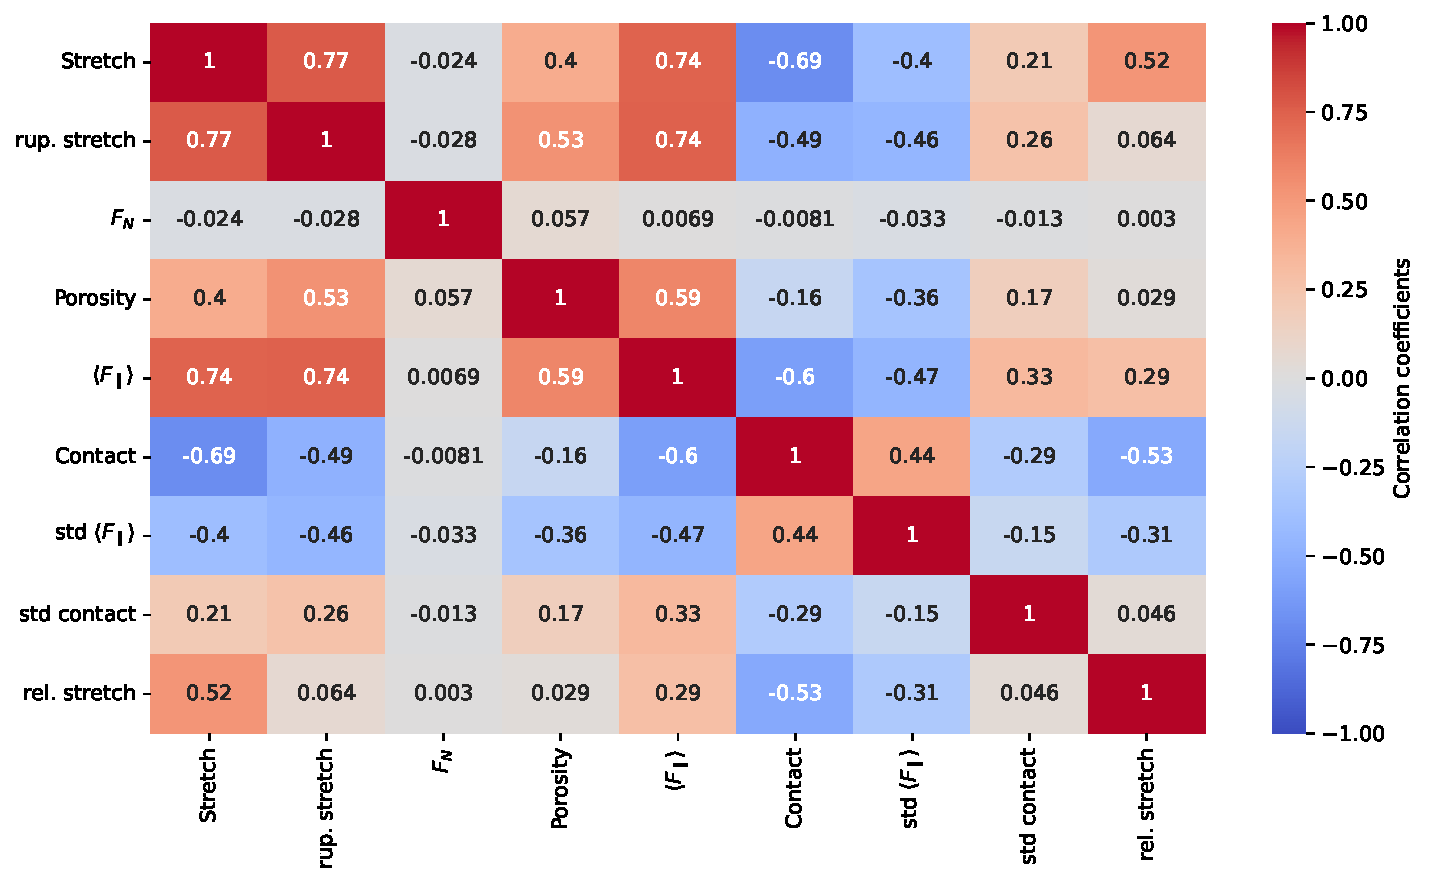
\includegraphics[width=\linewidth]{figures/ML/corrcoef_matrix.pdf}
  \caption{Pearson product-moment correlation coefficients for the full datset (see~\cref{tab:dataset_summary}).}
  \label{fig:corrcoef_matrix}
\end{figure}
From~\cref{fig:corrcoef_matrix} we especially notice that the mean friction
force $\langle F_{\parallel} \rangle$ has a significant positive correlation
with strain $(0.77)$ and porosity $(0.60)$. However, the relative strain, the
strain scaled by the rupture strain, has a weaker correlation of only 0.25.
This indicates that the correlation might be associated with the flexibility of
the configurations since these can be taken to higher absolute values of strain.
This is further supported by the fact that the mean friction and the rupture
strain are also strongly positively correlated $(0.78)$. From~\cref{fig:corrcoef_matrix} we also observe that the contact is negatively
correlated with the mean friction $(-0.67)$ and the strain value $(-0.74)$. This is generally consistent with the trend observed in the pilot study in~\cref{fig:multi_stretch} where the increasing strain was correlated with a decreasing contact and mainly increasing mean friction. However, we must note that the correlation coefficient is a measure of the quality of a forced linear fit on the data. Since we have observed a non-linear trend between friction and strain (\cref{fig:multi_stretch_mean_fric}) we should not expect any near 100 \% correlations. Additionally, we also notice that all correlations to normal load are rather low, which aligns well with the findings in the pilot study. 

\cref{fig:corr_vis} shows a visualization of the data (excluding
the pilot study configurations) for chosen variable pairs on the axes. This
provides a visual clue on some of the correlations and provides a qualitative
feeling for the diversity in various planes of the feature space that we
eventually will base our machine learning model on. We notice that the
honeycomb pattern is spanning a significantly larger range of strain, contact
and mean friction.


\begin{figure}[H]
  \centering
  \begin{subfigure}[t]{0.49\textwidth}
      \centering
      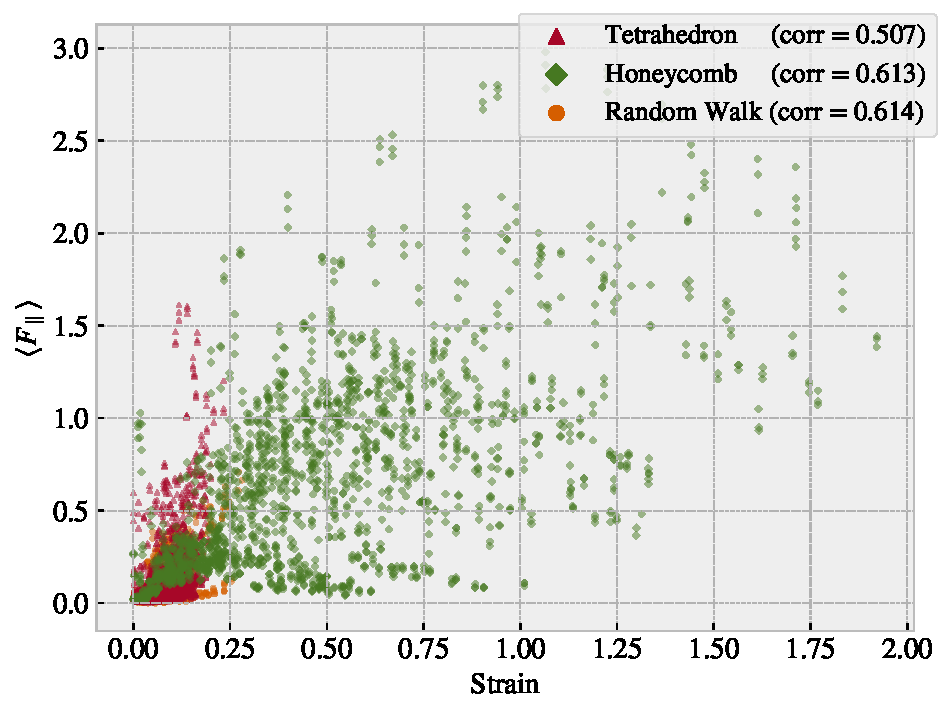
\includegraphics[width=\textwidth]{figures/ML/corr_stretch_Ff.pdf}
      \caption{}
      % \label{fig:}
  \end{subfigure}
  \hfill
  \begin{subfigure}[t]{0.49\textwidth}
      \centering
      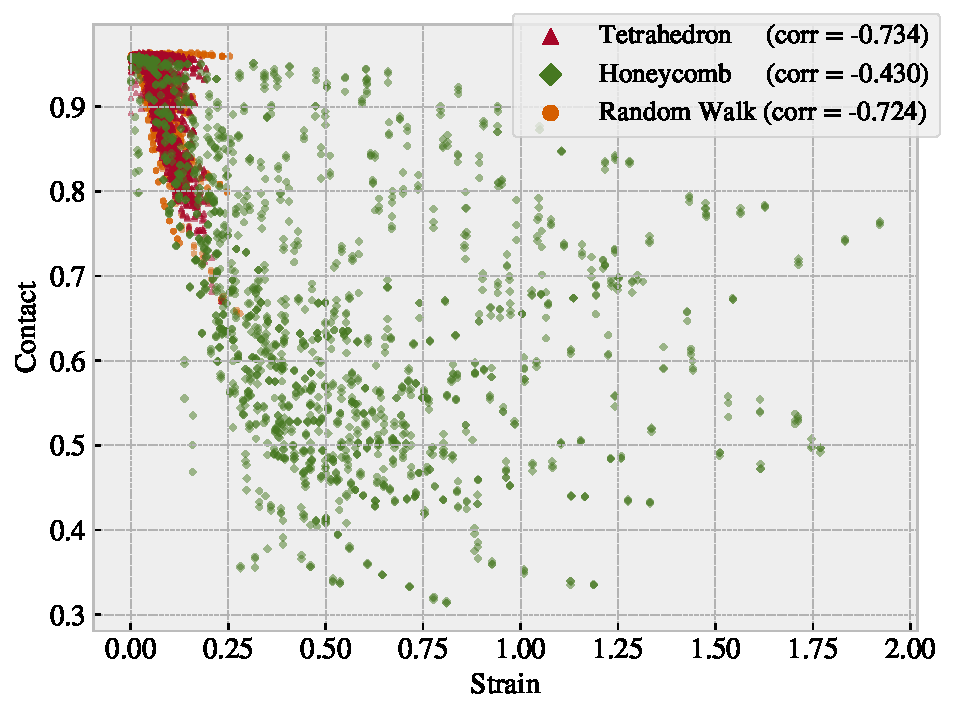
\includegraphics[width=\textwidth]{figures/ML/corr_stretch_contact.pdf}
      \caption{}
      % \label{fig:}
  \end{subfigure}
  \hfill
  \begin{subfigure}[t]{0.49\textwidth}
      \centering
      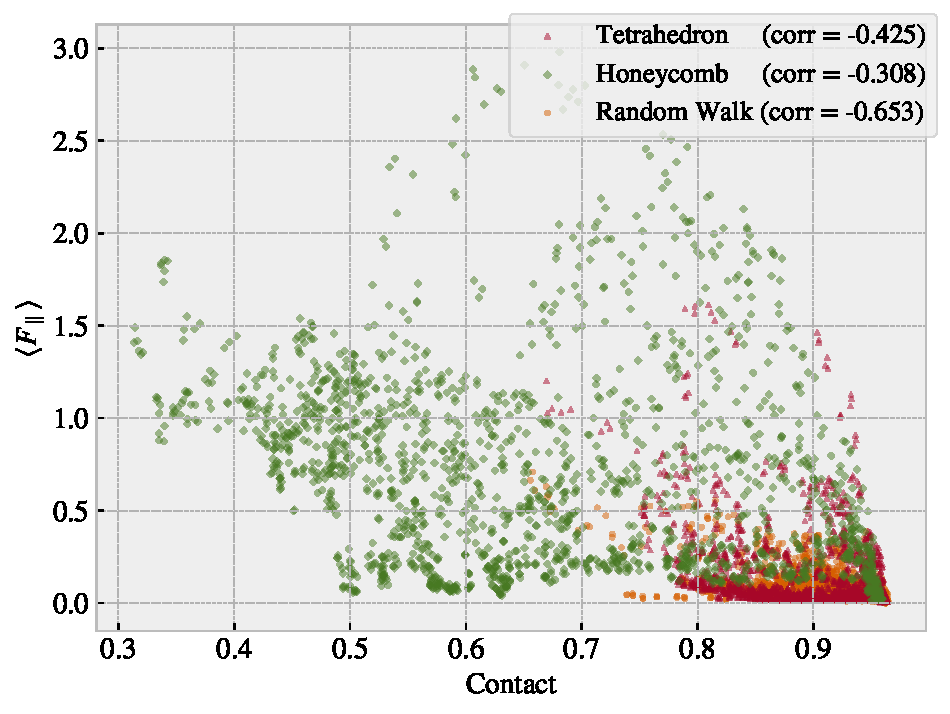
\includegraphics[width=\textwidth]{figures/ML/corr_contact_Ff.pdf}
      \caption{}
      % \label{fig:}
  \end{subfigure}
  \hfill
  \begin{subfigure}[t]{0.49\textwidth}
      \centering
      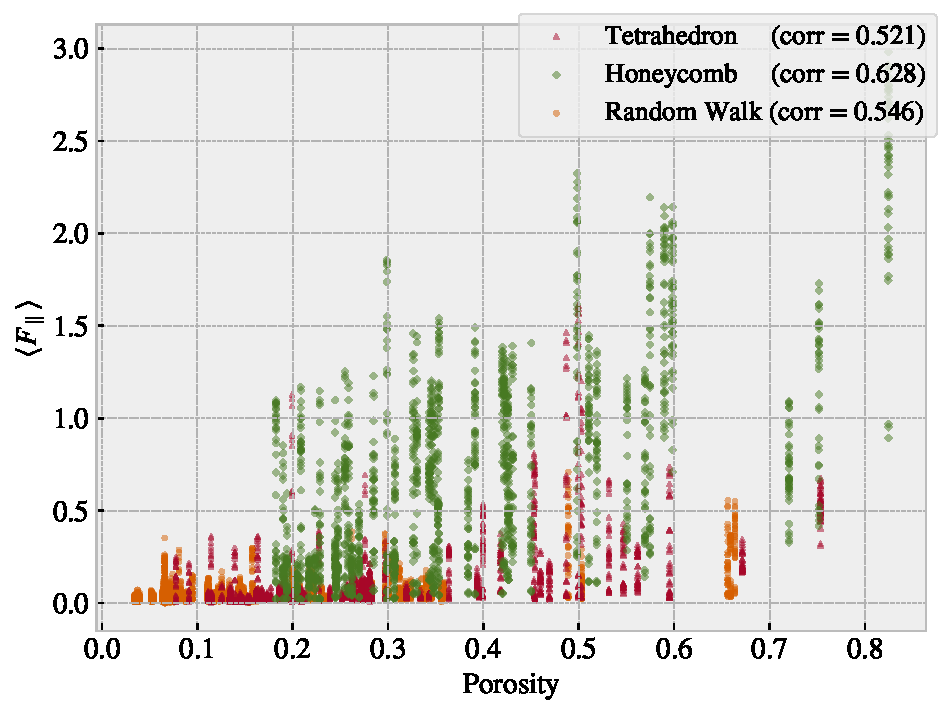
\includegraphics[width=\textwidth]{figures/ML/corr_porosity_Ff.pdf}
      \caption{}
      % \label{fig:}
  \end{subfigure}
  \hfill
     \caption{Scatter plot of the data sets Tetrahedron, Honeycomb and Random Walk (excluding the pilot study) for various variable combinations in order to visualize some chosen  correlations of interest and distributions in the data}
     \label{fig:corr_vis}
\end{figure}



\section{Properties of interest} 
In the pilot study (\cref{chap:pilot_study}) we found promising results for the idea of achieving a negative friction coefficient under the assumption of a system with coupled normal force and strain. Hence, we will consider this as a main property of interest for our further exploration. However, it is not obvious how one should rigorously quantify this. The friction coefficient is by our definition (\cref{eq:mu_def2}) given as the slope of the friction $F_f$ vs.\ normal force $F_N$ curve. Hence, for two data points $\{(F_{N,1}, F_{f,1}), (F_{N,2}, F_{f,2})\}$, $F_{N,1} < F_{N,2}$ we can evaluate the associated friction coefficient $\mu_{1,2}$ as 
\begin{align*}
  \mu_{1,2} = \frac{F_{f,2} - F_{f,1}}{F_{N,2} - F_{N,1}} = \frac{\Delta F_f}{\Delta F_N}.
\end{align*}
In the pilot study, it became apparent that the effects of friction under the
change of load is negligible in comparison to the effects related to strain $\varepsilon$.
Thus, by working under the assumption $F(F_N, \varepsilon) \sim F(\varepsilon)$ and a coupling $F_N
\propto R\cdot \varepsilon$ with linear coupling ratio $R$ we get 
\begin{align}
  \mu_{1,2}(\varepsilon_1, \varepsilon_2) = \frac{\Delta F_{f}(\varepsilon_1, \varepsilon_2)}{R(\varepsilon_2 - \varepsilon_1)} \propto \frac{\Delta F_{f}(\varepsilon_1, \varepsilon_2)}{\Delta \varepsilon}.
  \label{eq:mu_strain}
\end{align}
With this reasoning, we can in practice substitute load $F_N$ for strain
$\varepsilon$ in the expression for the friction coefficient of our coupled
system. This justifies the search for a negative slope on the friction-strain
curve since this can be related to a negative friction coefficient in our
proposed coupled system. The remaining question is then how to evaluate the
strength of this property. By definition, the minimum (most negative) slope
value would give the lowest friction coefficient. However, two data points with
a small $\Delta \varepsilon$, corresponding to a small denominator
in~\cref{eq:mu_strain}, would potentially lead to a huge negative slope value
without any significant decrease in friction. Hence, we choose to consider the
drop in friction with increasing strain as a better metric. Numerically we
compute this by locating the local maxima on the friction-strain curve and then
evaluating the difference to the succeeding local minima. The biggest difference
corresponds to the \textit{max drop} which serves as our indicator for a
negative friction coefficient. In this evaluation, we do not guarantee a
monotonic decrease of friction in the range of the biggest drop, but when
searching among multiple configurations this is considered a decent strategy to
highlight configurations of interest worthy of further investigation. In
addition to the biggest drop in friction, we also consider the minimum, $\min
F_{\text{fric}}$, and maximum, $\max F_{\text{fric}}$, friction along with the
maximum difference, $\max \Delta f_{\text{fric}} = \max F_{\text{fric}} - \min
F_{\text{fric}}$. The extrema of these four properties for each of the
categories: Tetrahedron, Honeycomb, Random walk and Pilot study, are summarized
in~\cref{tab:data_properties}. The corresponding strain profiles and
configurations are shown in~\crefrange{fig:PP_min}{fig:PP_max_drop} (excluding
the pilot study). The strain profiles for the full dataset are shown in
appendix~\ref {sec:data_stretch_profiles}. 

From the property comparison in~\cref{tab:data_properties} we find that both the
Tetrahedron and Honeycomb subsets contain improved candidates for each of the
property scores in comparison to the Tetrahedron $(7,5,1)$ and Honeycomb
$(2,2,1,5)$ examined in the pilot study. Overall, the Honeycomb pattern type is
still resulting in the highest scores for the maximum properties while the
minimum friction is still achieved by the non-cut sheet. This latter observation
reveals that our dataset does not provide any indication that friction can readily be reduced for a Kirigami sheet under strain. However, the improvement in the
remaining properties indicates that the dataset contains the necessary
information to provide a direction for further optimization of the maximum properties. Considering the Random walk we find that the max property scores are generally lower than that of the Tetrahedron and Honeycomb structures. However, since these are found to be on a comparable order of magnitude we argue that contain relevant information for populating configuration space with respect to machine learning training. The Random walk patterns also contribute with some immediate insight into the structures that we can associate with each of the properties of interest due to its increased diversity in comparison to the other patterns.

For the $\min F_{\text{fric}}$ top candidates (\cref{fig:PP_min}) we find that
the Random walk candidate has a rather cut density (low porosity) and with
vertical cuts. Since these cuts run parallel to the stretching direction one can
hypothesize that this minimizes the induced buckling effect which agrees with
the constant level of contact. For the minimum candidate for the Tetrahedron
pattern, we also observe a low decrease in contact, and in both these cases this
corresponds with a relatively flat friction-strain curve. When considering the
remaining friction-strain curve
throughout~\crefrange{fig:PP_min}{fig:PP_max_drop} we find a rising
friction-strain curve which is accompanied by a decreasing relative contact.
When looking at the Random walk 96 pattern, which is the top candidate for both
the $\max F_{\text{fric}}$ (\cref{fig:PP_max}) and $\max \Delta f_{\text{fric}}$
(\cref{fig:PP_max_diff}) property, we find a rather porous configuration with
mainly horizontal-orientated cuts. This has some structural reminiscence with the Honeycomb pattern. Finally, the best random walk candidate for the max drop category, Random walk 01, did not produce a big drop. We find that the contact area is decreasing with strain but not as strongly as seen for the other configurations. The configuration contains some slanted cuts which might be reminiscent of parts of the Tetrahedron pattern. 





\begin{table}[H]
  \begin{center}
  \caption{Evaluation of the properties of interest for our dataset.}
  \label{tab:data_properties}
  \begin{tabular}{| c | c | c | c | c |} \hline
  \textbf{Tetrahedron} & Configuration & Strain & Value [nN] & Hon. $(2,2,1,5)$ [nN]  \\ \hline
  $\min F_{\text{fric}}$ & $(3,9,4)$ &  0.0296 & 0.0067 & 0.0262 \\ \hline
  $\max F_{\text{fric}}$ & $(5,3,1)$ & 0.1391 & 1.5875 & 0.8891 \\ \hline
  $\max \Delta F_{\text{fric}}$  & $(5, 3, 1)$ & $[0.0239, 0.1391]$ & 1.5529 & 0.8603  \\ \hline
  max drop & $(5,3,1)$ & $[0.1391, 0.1999]$ & 0.8841 & 0.5098 \\ \hline
  \multicolumn{5}{c}{} \\ \hline
  \textbf{Honeycomb} & Configuration & Strain & Value [nN]  & Tetra. $(7,5,1)$ [nN]  \\ \hline
  $\min F_{\text{fric}}$ & $(2, 5, 1, 1)$ &  0.0267 & 0.0177 & 0.0623 \\ \hline
  $\max F_{\text{fric}}$ & $(2, 1, 1, 1)$ & 1.0654 & 2.8903 & 1.5948 \\ \hline
  $\max \Delta F_{\text{fric}}$  & $(2, 1, 5, 3)$ & $[0.0856, 1.4760]$ & 2.0234 & 1.5325 \\ \hline
  max drop & $(2, 3, 3, 3)$ & $[0.5410, 1.0100]$ & 1.2785 & 0.9674\\ \hline
  \multicolumn{5}{c}{} \\ \cline{1-4}
  \textbf{Random walk} & Configuration & Strain & Value [nN] & \multicolumn{1}{c}{} \\ \cline{1-4}
  $\min F_{\text{fric}}$ & 12 &  0.0562 & 0.0024& \multicolumn{1}{c}{} \\ \cline{1-4}
  $\max F_{\text{fric}}$ & 96 & 0.2375 & 0.5758 & \multicolumn{1}{c}{} \\ \cline{1-4}
  $\max \Delta F_{\text{fric}}$  & 96 & $[0.0364, 0.2375]$ & 0.5448 & \multicolumn{1}{c}{} \\ \cline{1-4}
  max drop & 01 & $[0.0592, 0.1127]$ & 0.1818 & \multicolumn{1}{c}{} \\ \cline{1-4}
  \multicolumn{5}{c}{} \\ \cline{1-4}
  \textbf{Pilot study} & Configuration & Strain & Value [nN]  & \multicolumn{1}{c}{} \\ \cline{1-4}
  $\min F_{\text{fric}}$ & No cut & 0.2552 & 0.0012 & \multicolumn{1}{c}{} \\ \cline{1-4}
  $\max F_{\text{fric}}$ & Honeycomb & 0.7279 & 1.5948 & \multicolumn{1}{c}{} \\ \cline{1-4}
  $\max \Delta F_{\text{fric}}$  & Honeycomb & 0.7279 & 1.5325 & \multicolumn{1}{c}{} \\ \cline{1-4}
  max drop & Honeycomb & $[0.7279, 1.0463]$ & 0.9674 & \multicolumn{1}{c}{} \\ \cline{1-4}
\end{tabular}
\end{center}
\end{table}



\begin{figure}[H]
  \centering
  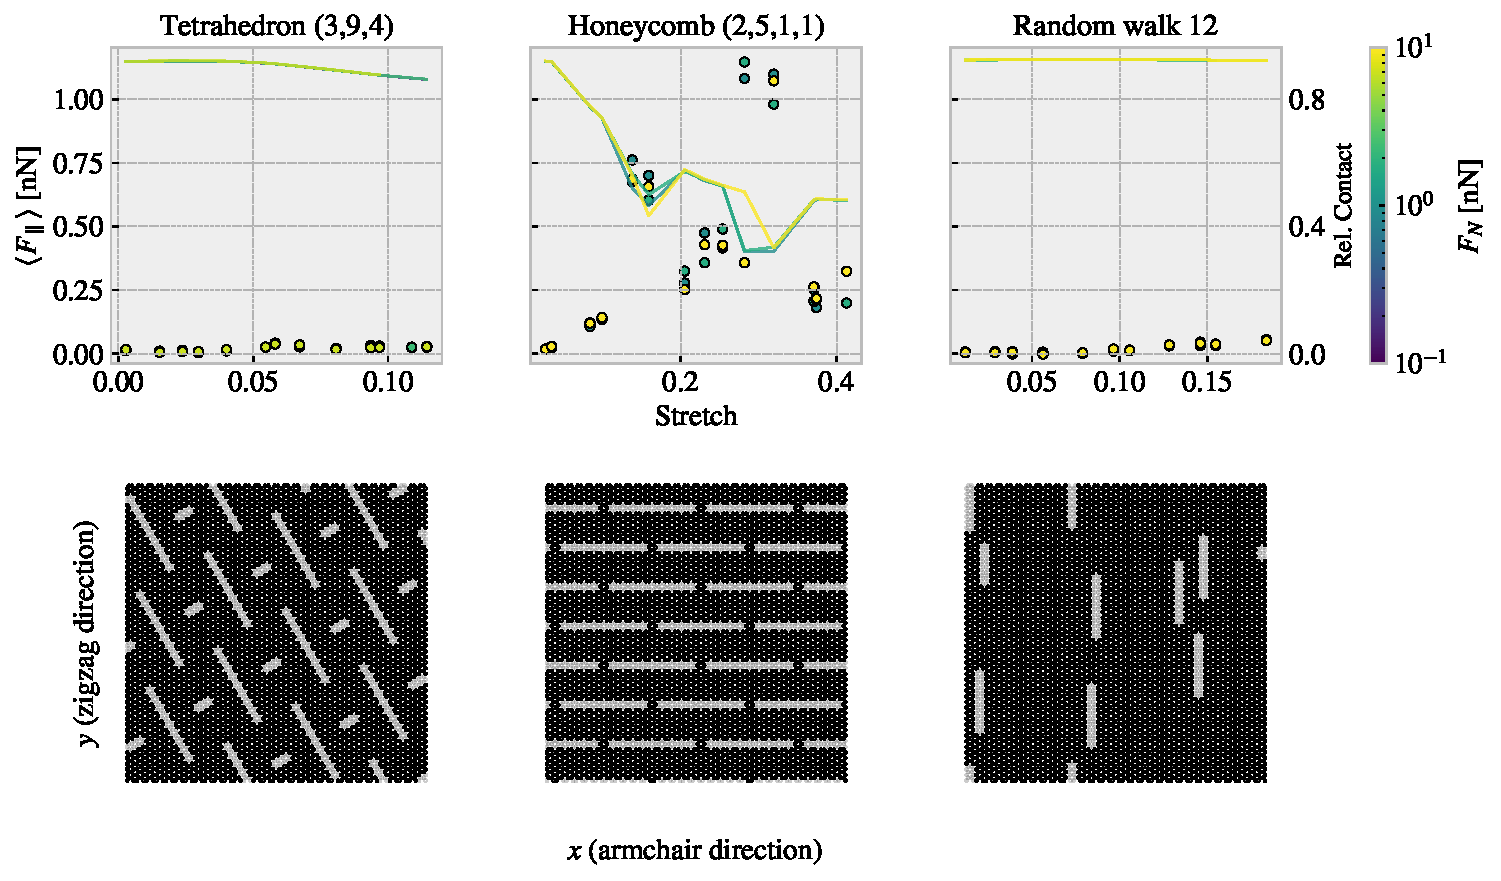
\includegraphics[width=\linewidth]{figures/stretch_profiles/PP_min.pdf}
  \caption{Minimum friction: Configurations corresponding to the minimum friction.}
  \label{fig:PP_min}
\end{figure}


\begin{figure}[H]
  \centering
  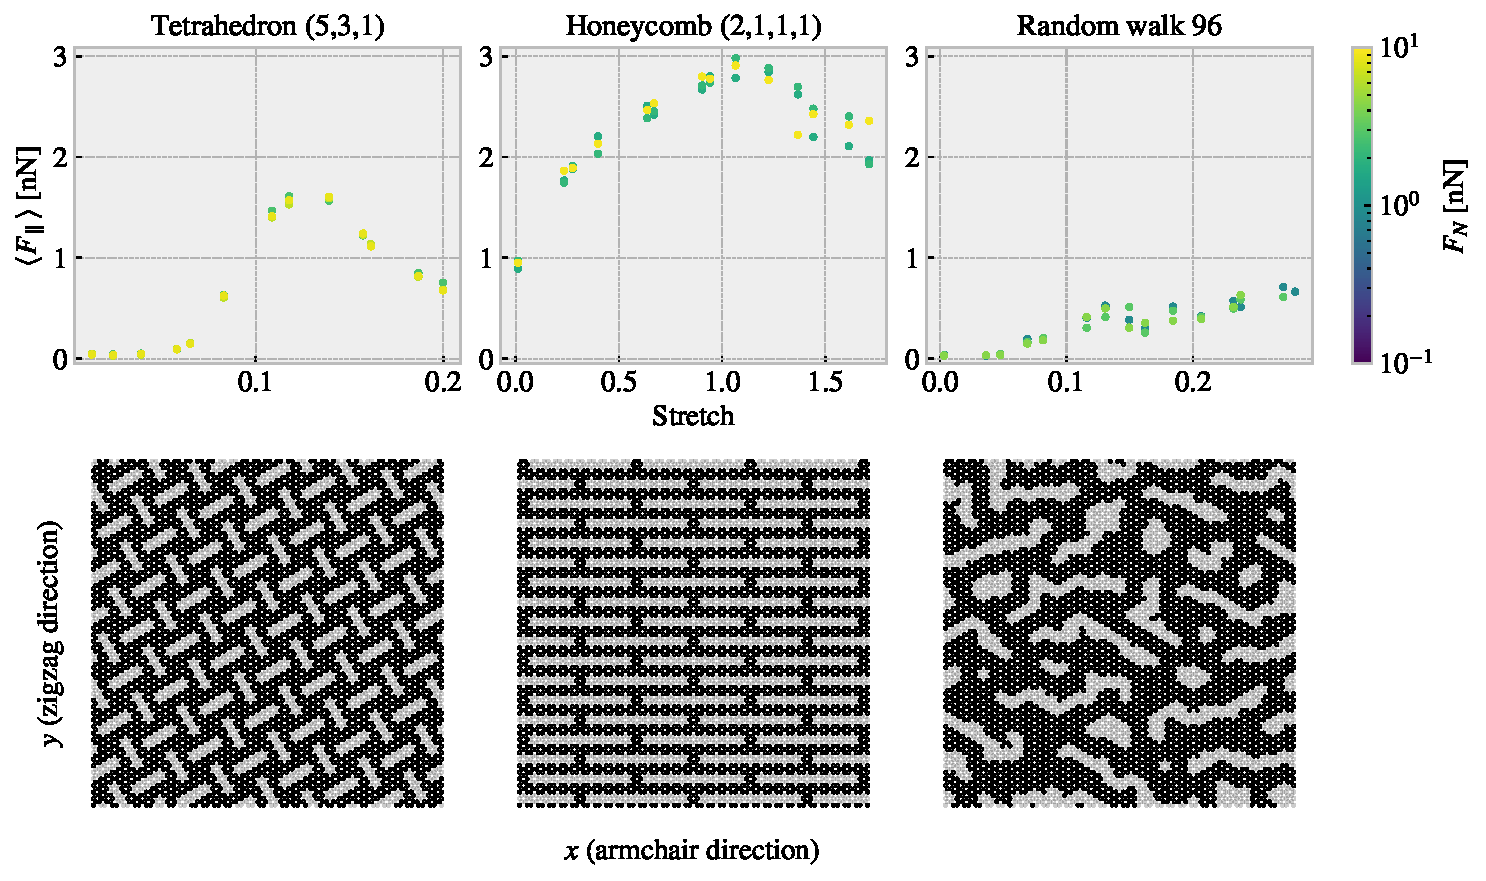
\includegraphics[width=\linewidth]{figures/stretch_profiles/PP_max.pdf}
  \caption{Maximum friction: Configurations corresponding to the maximum friction.}
  \label{fig:PP_max}
\end{figure}


\begin{figure}[H]
  \centering
  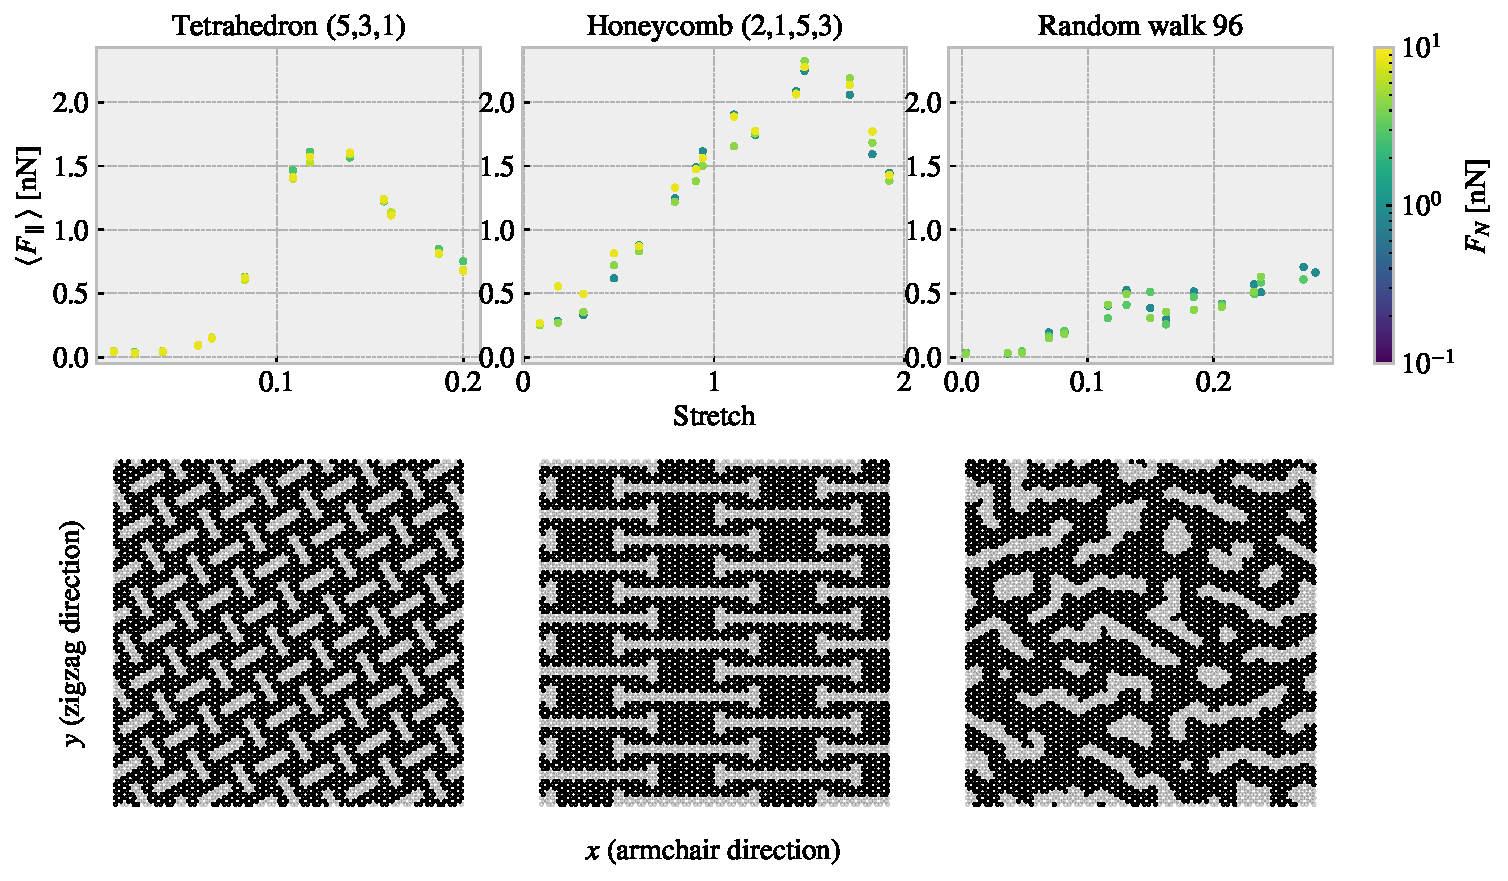
\includegraphics[width=\linewidth]{figures/stretch_profiles/PP_max_diff.pdf}
  \caption{Maximum Difference: Configurations corresponding to the biggest difference in friction in the dataset for each pattern.}
  \label{fig:PP_max_diff}
\end{figure}  

\begin{figure}[H]
  \centering
  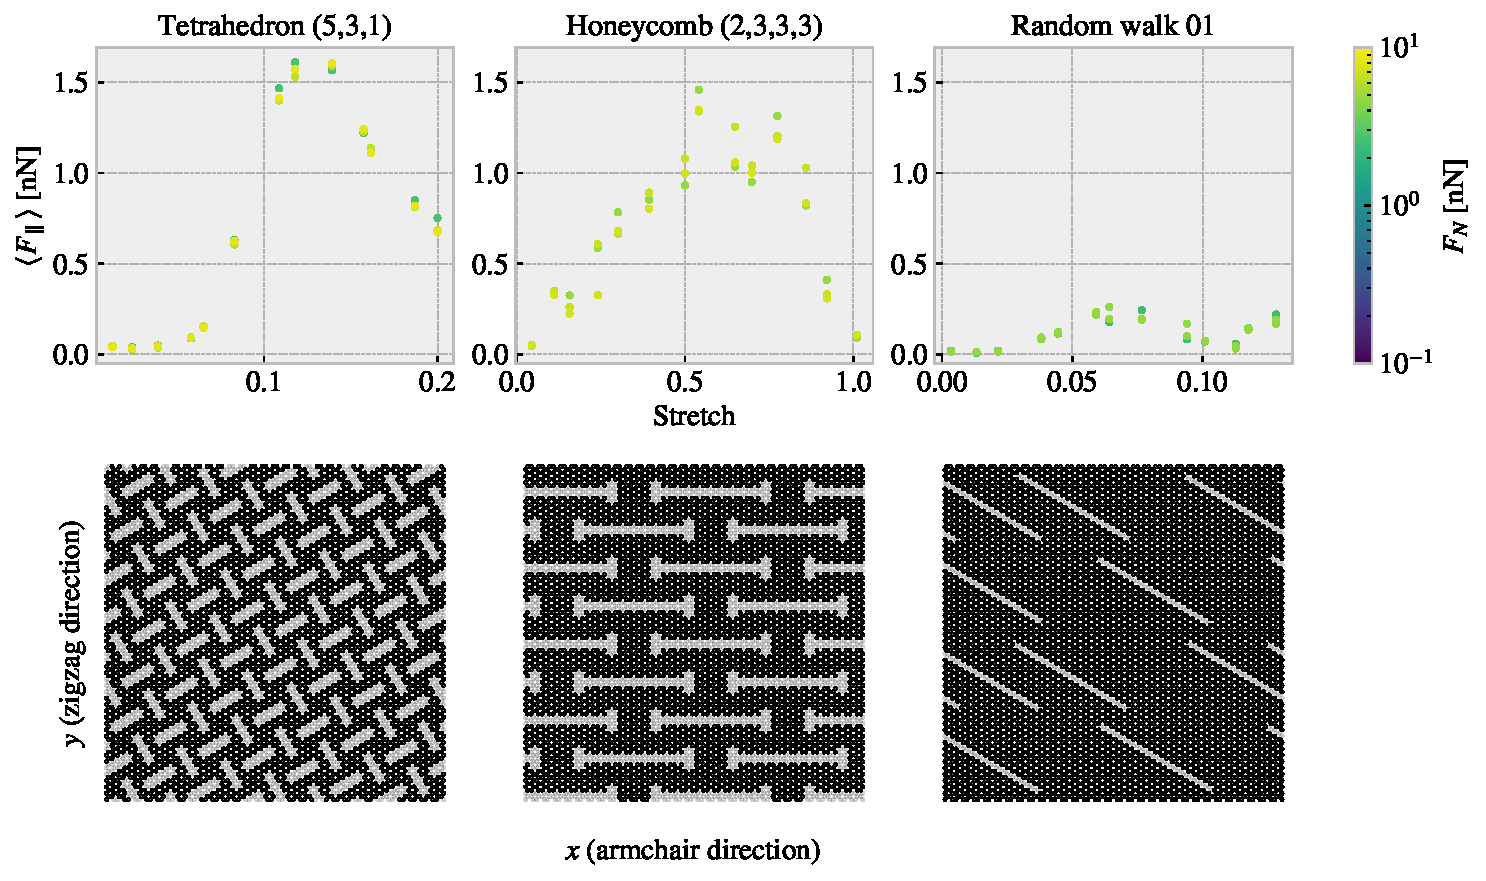
\includegraphics[width=\linewidth]{figures/stretch_profiles/PP_max_drop.pdf}
  \caption{Maximum drop: Configuratiosn corresponding to the biggest friction drop in the dataset for each pattern.}
  \label{fig:PP_max_drop}
\end{figure}  









\section{Machine learning}\label{eq:ML}
Given the \acrshort{MD}-based dataset we investigate the possibilities of training a machine learning model to predict the friction behavior from a given Kirigami configuration, strain and load. 

\subsection{Architecture}
Due to the spatial dependencies in the Kirigami configurations, we use a convolutional neural network (\acrshort{CNN}). Similar studies which predict mechanical properties for graphene sheets have used a VGGNet style network, Hanakata et al.~\cite{PhysRevLett.121.255304, PhysRevResearch.2.042006} and Wan et al.~\cite{graphene/hBN}, which we adopt for this study as well. The VGGNet-16 architecture illustrated in~\cref{fig:VGGNet16} shows the key features that we will include:
\begin{itemize}
  \item The image is processed through a series of $3 \times 3$ convolutional filters (the smallest size capable of capturing spatial dependencies) using a stride of 1 with an increasing number of channels throughout the network. We use padding to conserve the spatial size during a convolution. Each convolutional layer is followed by a ReLU activation function. 
  \item The spatial dimensions are reduced by a max pooling, filter size $2 \times 2$ and a stride of 2, which halves the spatial resolution each time. 
  \item The latter part of the network consists of a fully connected part using the ReLu activation as well. The transition from the convolutional to the fully connected part is achieved by applying a filter with the same dimensions as the last convolutional feature map. This essentially performs a linear mapping from the spatial output to the fully connected layer with the number of channels corresponding to the nodes in the first fully connected layer.
\end{itemize}

% Remember the padding
\begin{figure}[H]
  \centering
  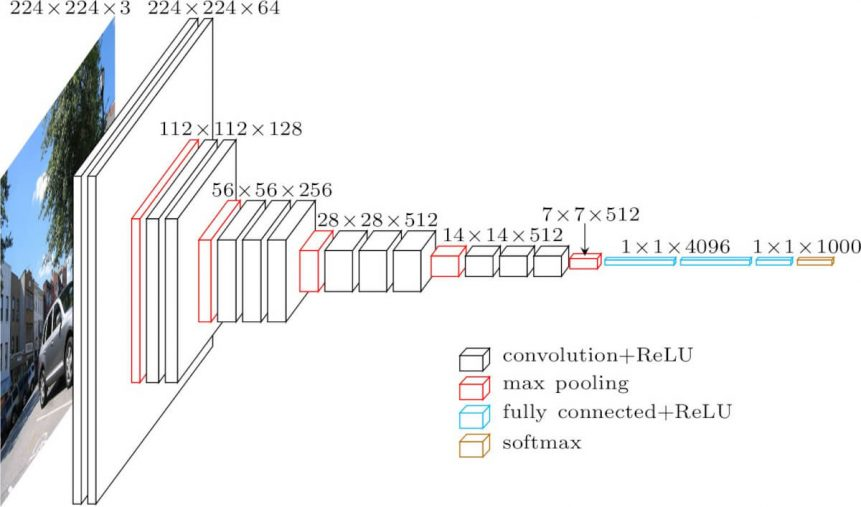
\includegraphics[width=0.7\linewidth]{figures/ML/VGGNet16.jpg}
  \caption{\hl{VGGNet-16}. Source \url{https://neurohive.io/en/popular-networks/vgg16/}.}
  \label{fig:VGGNet16}
\end{figure}

We deviate from the VGGNet-16 architecture by including batch normalization and restricting ourselves to setting up the convolutional part of the network in terms of the blocks: (Convolution $\to$ Batch normalization $\to$ ReLU $\to$ Max pooling). Similarly, we define a fully connected block by two elements (Fully connected $\to$ ReLU) which match the VGGNet model. Hanakata et al.\ and Wan et al.\ used a similar architecture with the parameters 
\begin{align*}
  \text{Hanakata et al.~\cite{PhysRevLett.121.255304}} & \qquad C16 \ C32 \ C64 \ D64, \\ 
  \text{Wan et al.~\cite{graphene/hBN}} & \qquad C16 \ C32 \ D32 \ D16,
\end{align*}
where $C$ denotes a convolutional block with the number denoting the number of channels, and $D$ a fully connected (dense) block with the number denoting the number of nodes. For the process of determining a suiting complexity for the architecture, we adopt the approach by Wan et al.~\cite{graphene/hBN} who used a ``staircase'' pattern for combining convolutional and fully connected blocks. By defining a starting number of channels $S$ and network depth $D$ we fill the first half of the network layers with convolutional blocks, doubling in channel number for each layer, and the latter half with fully connected blocks having the number of nodes decrease in a reverse pattern. For instance, the architecture $S4D8$ will take the form
\begin{align*}
  \text{Input} \to \underbrace{\overbrace{C4}^{S \ = \ 4}C8 \ C16 \ C32 \ D32 \ D16 \ D8 \ D4}_{D \ = \ 8} \to \text{Output}.
\end{align*} 
This provides a simple description where $S$ and $S$ can be varied systematically for a grid search over architecture complexity. 


\subsection{Data handling}
\subsubsection{Input}
We use three variables as input: Kirigami configuration, strain of the sheet
and applied normal load. The configuration is given as a two-dimensional input by the binary matrix while the strain and load are both scaler values. This gives rise to two different options for the data structure:
\begin{enumerate}
  \item Expand the scalar values (strain and load) into 2D matrices of the same
  size as the Kirigami configuration by copying the scaler value to all matrix coordinates. This can then be merged into an image of three channels used as a single input.  
  \item Pass only the Kirigami configuration through the convolutional part of the network and introduce the remaining scalar values into the fully connected part of the network halfway in. 
\end{enumerate}
Both options utilize the same data, but the latter option is more directed towards independent processing of the data while the first makes for an intertwined ude of the configuration, strain and load. We implemented both options but found immediately that option 1 was producing the most promising results during the initial test runs, and thus we settled for this data structure. 

\subsubsection{Output}
For the output, we are mainly concerned with mean friction and the rupture
detection. In combination, this will make the model able to produce a friction-strain curve with an estimated stopping point as well. However, in order to retain the option to explore other relations in the data we include the maximum friction, relative contact, porosity and rupture strain in the output as well. Notice that we weigh the importance of these output variables differently in the loss as described in~\cref{sec:loss}. 


\subsubsection{Data augmentation}
In order to increase the utility of the available data one can introduce data augmentation. For most classification tasks this usually includes distortions such as color shifts, zoom, flip etc. However, such distortions are only valid since the classification network should still classify a cat as a cat even though it is suddenly a bit brighter or flipped upside down. For our problem, we can only use augmentation that matches a physical symmetry. Such a symmetry exists for reflection across the y-axis. We cannot use a reflection across the
x-axis as the sheet is sliding in a positive y-direction. This would correspond to a change in the sliding direction which we cannot expect to be fully symmetric. 


\subsection{Loss}\label{sec:loss}
The output contains two different types of variables: scalar values and a binary value (rupture). For the scalar values we use the Mean Squared Error (\acrshort{MSE})~\cref{eq:MSE} and for the binary output, we use binary cross entropy~\cref{eq:BSE}. We calculate the total loss as a weighted sum of the loss associated with
each variable
\begin{align*}
  L_{tot} = \sum_{v} W_v\cdot L_v.
\end{align*}
We choose the weights to be $1/2$ for the mean friction and $1/10$ for the
remaining 5 variables, thus sharing the loss evenly for the remaining 50\% of the weight. During the introductory phase of the training, we tried different settings for these weights, but we found that the results varied little. Hence, we concluded that this was of minor importance and stuck to the values defined above.

\subsection{Hypertuning}
% Show overfitting curve for some of the training results?
For the hypertuning we focus on architecture complexity, learning rate, momentum and weight decay. We will use the ADAM optimizer with the initial default values of $beta_1 = 0.9, \beta_2 = 0.999$ and zero weight decay (we will change momentum $\beta_1$ and weight decay). We use a batch size of 32 and train the model for a maximum of 100 epochs while storing the best model based on the validation scores.
Since the learning rate is considered to be one of the most important hyperparameters we will determine a suitable choice for the learning rate using the learning rate range test for each of the two major grid searches:
\begin{enumerate}
  \item Architecture complexity grid search of $S$ vs.\ $D$ with individually chosen learning rates for each complexity combination.
  \item Momentum vs.\ weight decay grid search with learning range chosen with regard to each momentum setting.
\end{enumerate}
We consider first the architecture complexities in the range $S \times D =
\{2,4,8,16,32,64,128,256\} \times \{4,6,8,10,12,14\}$. For each architecture
complexity, we perform an initial learning rate range test and determine the suitable choice as the point for which the validation loss decreases most rapidly. The learning rate is increased exponentially within the range \num{e-7} to 10 with increments for each training batch iteration. This is done for just a single epoch where a batch size of 32 yields a total of 242 increments. This corresponds to an exponent increment of approximately $1/30$ giving a relative increase $10^{1/30} \sim 108\%$ per batch iteration. The learning rate range test is presented in~\cref{fig:LR_range} for various model complexities. We notice that the suggested learning rate decreases with an increasing number of model parameters. This decrease is further independent of the specific relationship between $S$ and $D$.

\begin{figure}[H]
  \centering
  \begin{subfigure}[t]{0.49\textwidth}
      \centering
      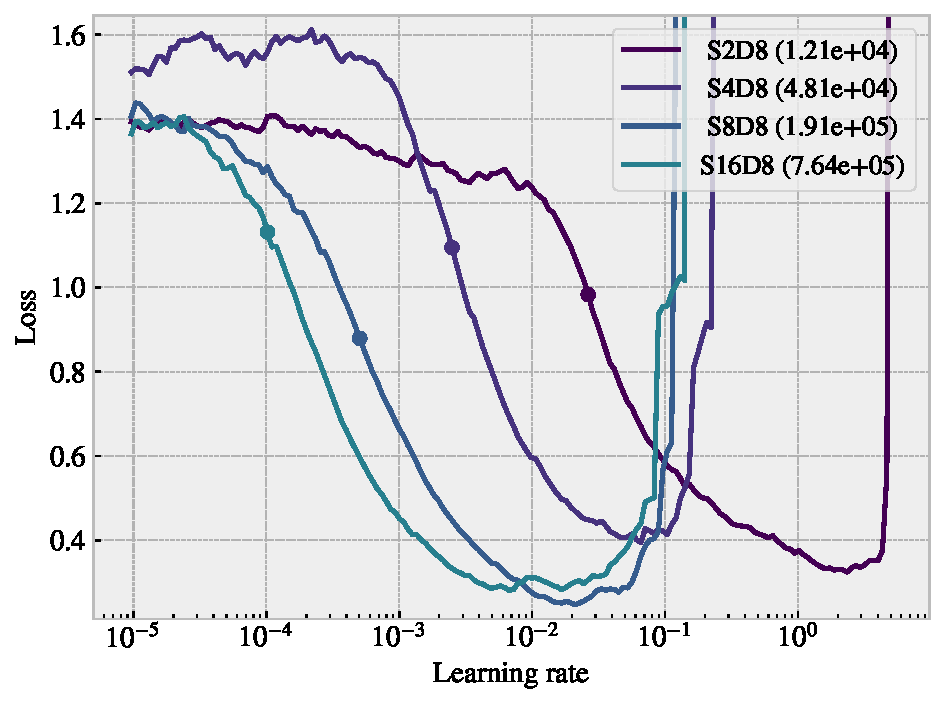
\includegraphics[width=\textwidth]{figures/ML/LR_range_specific.pdf}
      \caption{}
      % \label{fig:}
  \end{subfigure}
  \hfill
  \begin{subfigure}[t]{0.49\textwidth}
      \centering
      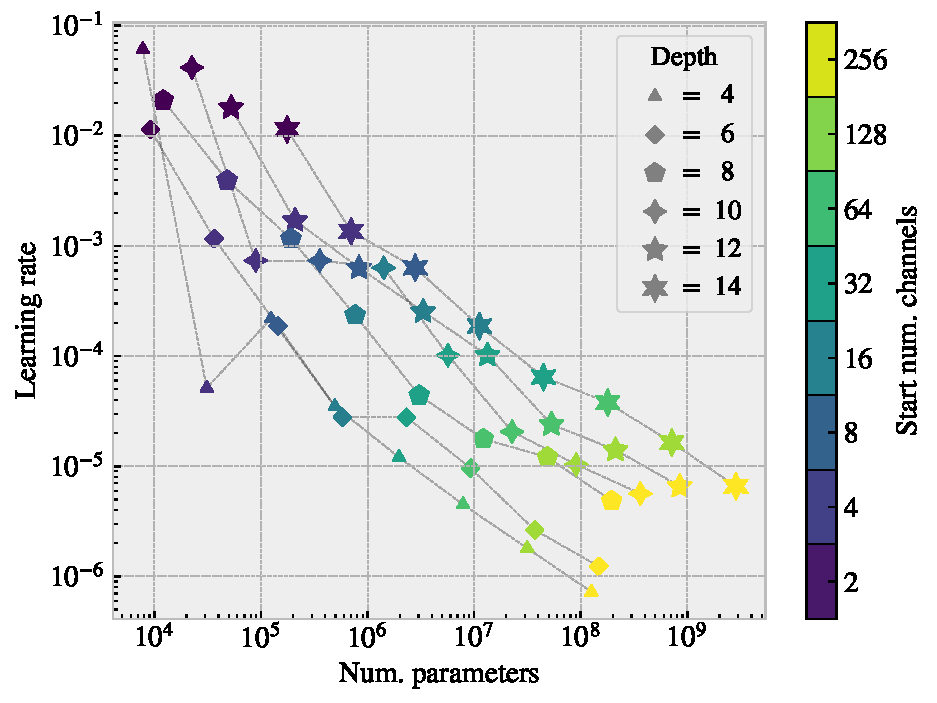
\includegraphics[width=\textwidth]{figures/ML/LR_range_full.pdf}
      \caption{}
      % \label{fig:}
  \end{subfigure}
  \hfill
  \caption{Learning rate range test for various model complexities. We increase the learning rate exponentially from num{e-7} to 10 during one epoch corresponding to an exponent increment of roughly $1/30$ per batch iteration. $(a)$ shows a few examples of the training loss history as a function of the learning rate. The exemplary architectures are S[2, 16]D8 with the corresponding number of model parameters shown in parentheses in the legend. The dot indicates the suggested learning rate at the steepest decline of the slope. $(b)$ shows the full results of suggested learning rates depending on the number of model parameters with color coding differentiating the number of start channels and marker types differentiating different model depths. }
  \label{fig:LR_range}
\end{figure}
With the use of the suggested learning rates from~\cref{fig:LR_range} we perform
a grid search over the corresponding $S$ and $D$ parameters. We evaluate both
the validation loss and the mean friction $R_2$ score for the validation data which is shown in~\cref{fig:A_search_perf} together with the best epoch and the number of model parameters. Additionally, we evaluate the mean friction $R_2$ score for a selected set of configurations. This set consists of the top 10 configurations with respect to the max drop property for the Tetrahedron and Honeycomb patterns respectively. This is done as a way of evaluating the performance on the non-linear strain curves which we immediately found to be the more difficult trend to capture. The selected evaluation is shown in~\cref{fig:A_search_compare}. Note that these configurations already are a part of the full dataset and thus the data points related to these configurations are most likely present in both the training and the validation data set. Hence, the performance must be considered in conjunction with the actual validation performance in~\cref{fig:A_search_perf}.

\begin{figure}[H]
  \centering
  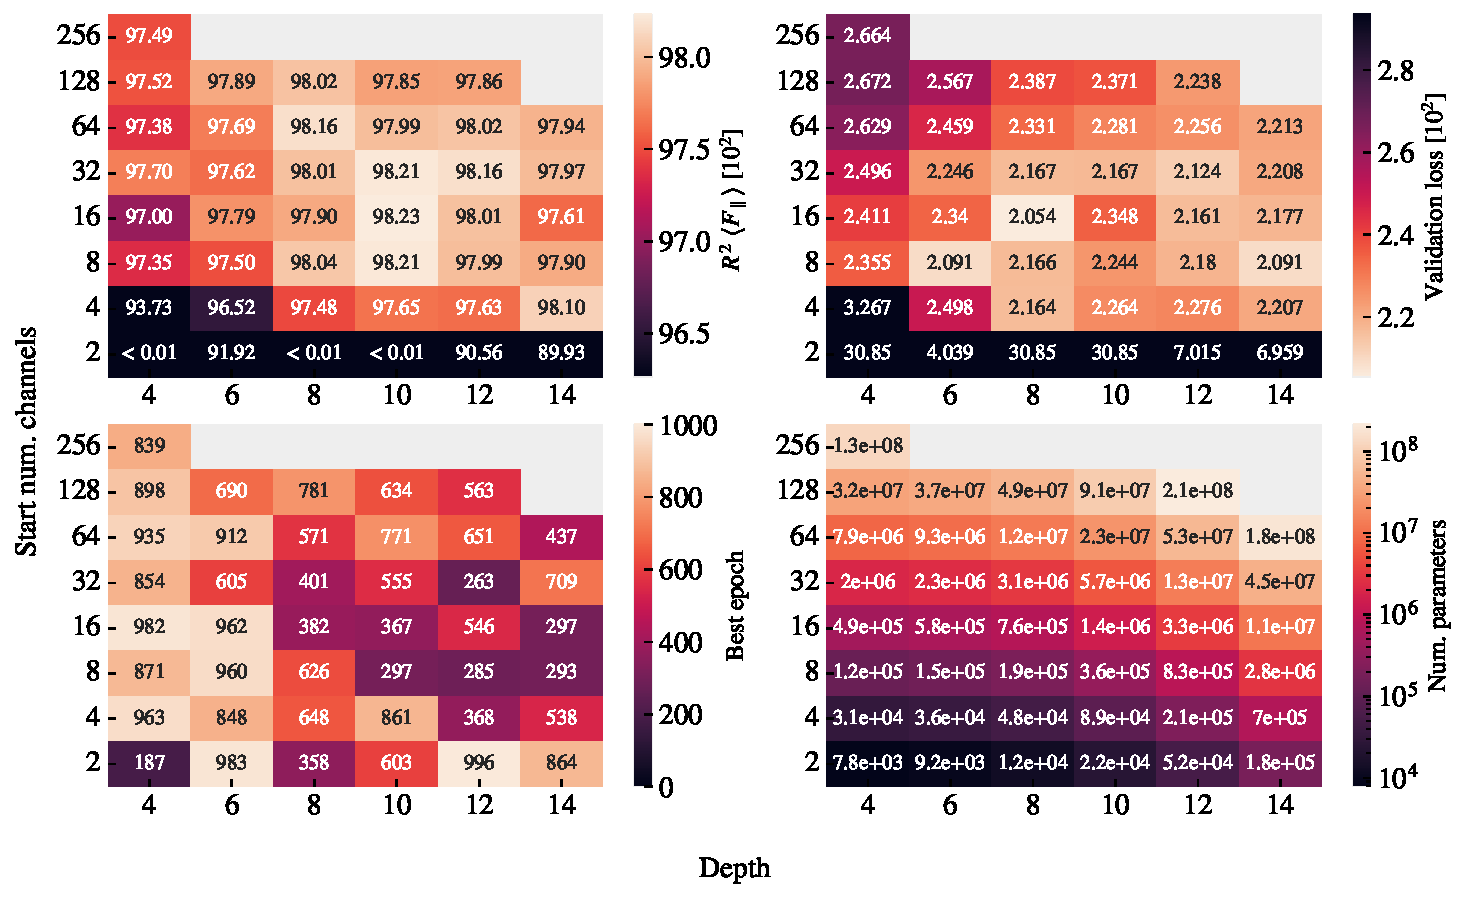
\includegraphics[width=\linewidth]{figures/ML/A_search_perf.pdf}
  \caption{Architecture search.}
  \label{fig:A_search_perf}
\end{figure}  

\begin{figure}[H]
  \centering
  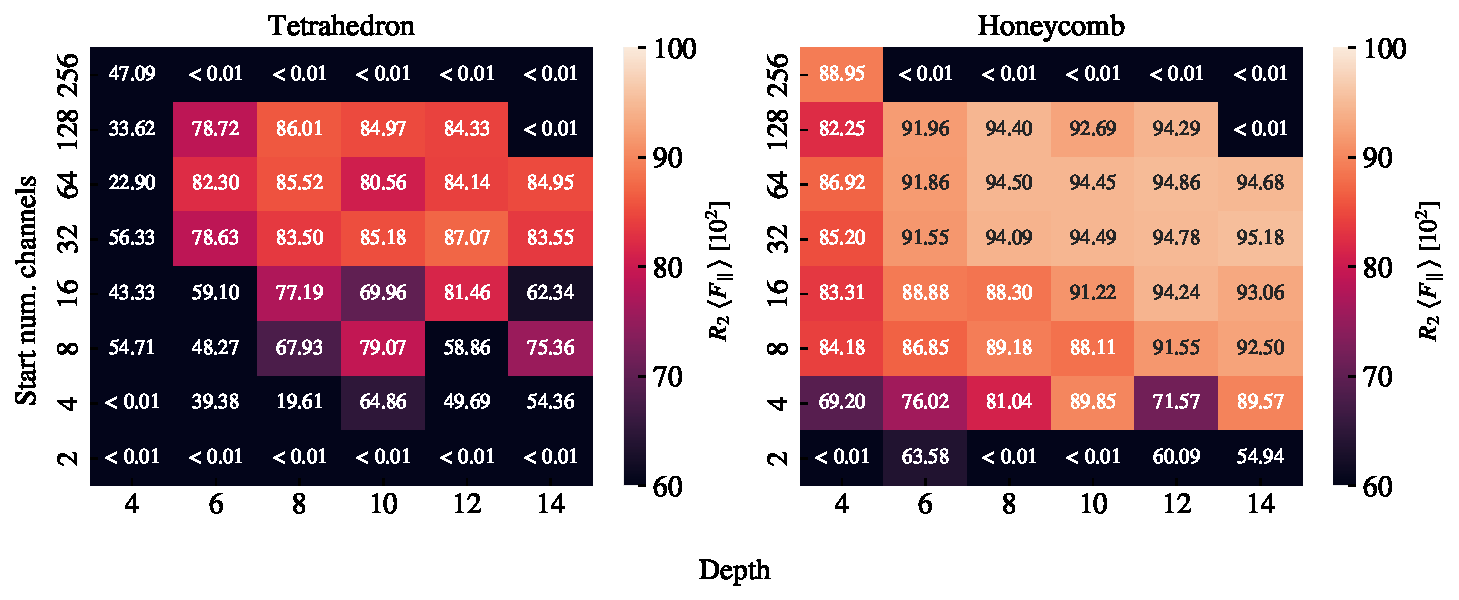
\includegraphics[width=\linewidth]{figures/ML/A_search_compare_perf}
  \caption{Selected pseudo validation set. \hl{Fix the missing grey fields in the top which are replaced by < 0.01.}}
  \label{fig:A_search_compare}
\end{figure}  

From the validation scores in~\cref{fig:A_search_perf}, looking at both the loss and the $R^2$ scores, we find that models
S(8-32)D(8-12) generally give the best performance. When looking at the best epoch we find that models of low depth result in a later best epoch which is compatible
with underfitting. As the depth is increased we find more models with a lower
best epoch, in the range $\sim [300, 600]$, which on the other hand suggest
cases of overfitting. Since our training stores the best model during training,
we do not have to worry too much about overfitting, but we can take this
transition from underfitting to overfitting as a sign that our search is
conducted in an appropriate complexity range. When consulting the evaluation on the
selected set in~\cref{fig:A_search_compare} we find
significantly lower $R_2$ scores, especially for the Tetrahedron pattern. Considering, that some of these data points are also present in the training data, this shows clearly that these configurations are more challenging to predict. While the peak $R_2$ value for the validation score in~\cref{fig:A_search_perf} was found for the model S16D10 model (98.23 \%) the selected set test shows a slight preference for more complexity in the model. In the Tetrahedron selected set grid search, we find the best model to be S32D12, with an $R_2$ score of $\sim 87 \%$. This model choice is more or less compatible with the overall performance as it is among the top candidates for the $R_2$ score and loss in~\cref{fig:A_search_perf} and the $R_2$ score for the Honeycomb pattern in~\cref{fig:A_search_compare} as well. Hence, we settle on this architecture. 

Next, we consider momentum $m$ and weight decay $\lambda$ in the range $m \in
[0.85, 0.99]$ and $\lambda \in [0, \num{1e-2}]$. For each choice of momentum, we
perform a learning rate range test. We propose two learning rate schemes: A
constant learning rate as used until this point and a one-cycle policy. In the
one-cycle policy, we set a maximum bound for the learning rate and start from a
factor $1/20$ of this bound and increase towards the maximum bound during the
first 30\% of the training. For the final 70\% of training, we decrease towards
a final minimum given as a factor $1e-4$ of the maximum bound. The increase and
decrease are done by a cosine function. The suggested learning rate for the
constant learning rate scheme is once again determined by the steepest slope on
the loss curve while the maximum bound used for the one-cycle policy is
determined as the point just before divergence. We find that the minimum point
on the loss curve is a suitable choice that approaches the diverging point
without getting too close and causing instabilities. The learning rate range
test for momentum is shown in~\cref{fig:LR_range_mom}. We observe generally that
a higher momentum corresponds to a higher suggested learning rate for both
schemes. Using these results we perform a grid search of momentum and weight
decay. We examine again the validation loss and validation mean friction $R_2$
score in addition to the friction mean $R_2$ score for the selected set of
Tetrahedron and Honeycomb patterns. This is shown for the constant learning rate
scheme in~\cref{fig:mom_weight_search_constant} and for the cyclic scheme
in~\cref{fig:mom_weight_search_cyclic}.

\begin{figure}[H]
  \centering
  \begin{subfigure}[t]{0.49\textwidth}
      \centering
      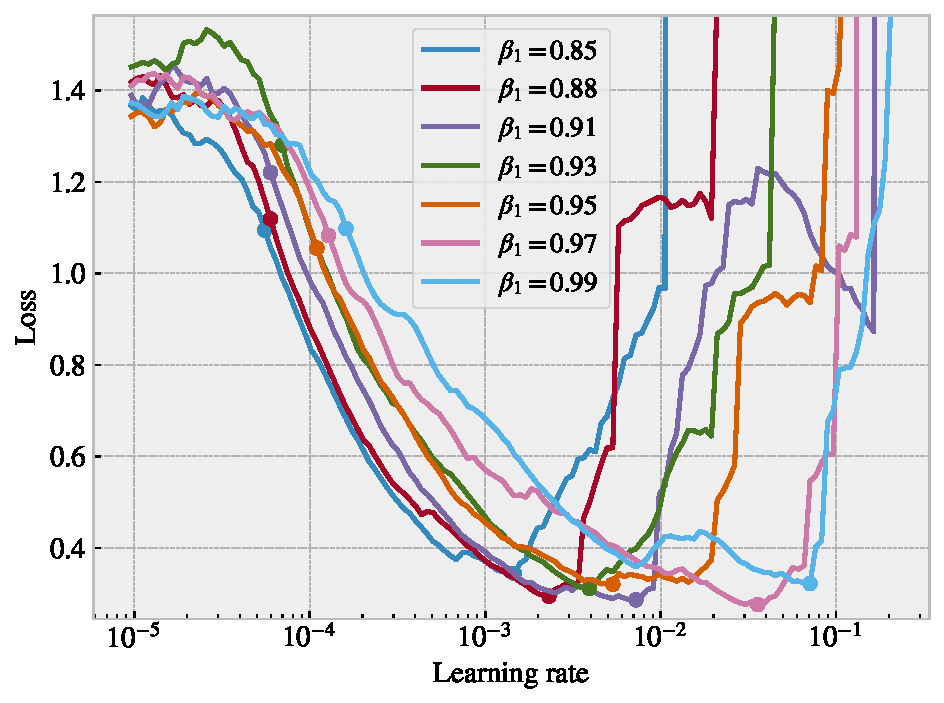
\includegraphics[width=\textwidth]{figures/ML/LR_momentum_test_a.pdf}
      \caption{}
      % \label{fig:}
  \end{subfigure}
  \hfill
  \begin{subfigure}[t]{0.49\textwidth}
      \centering
      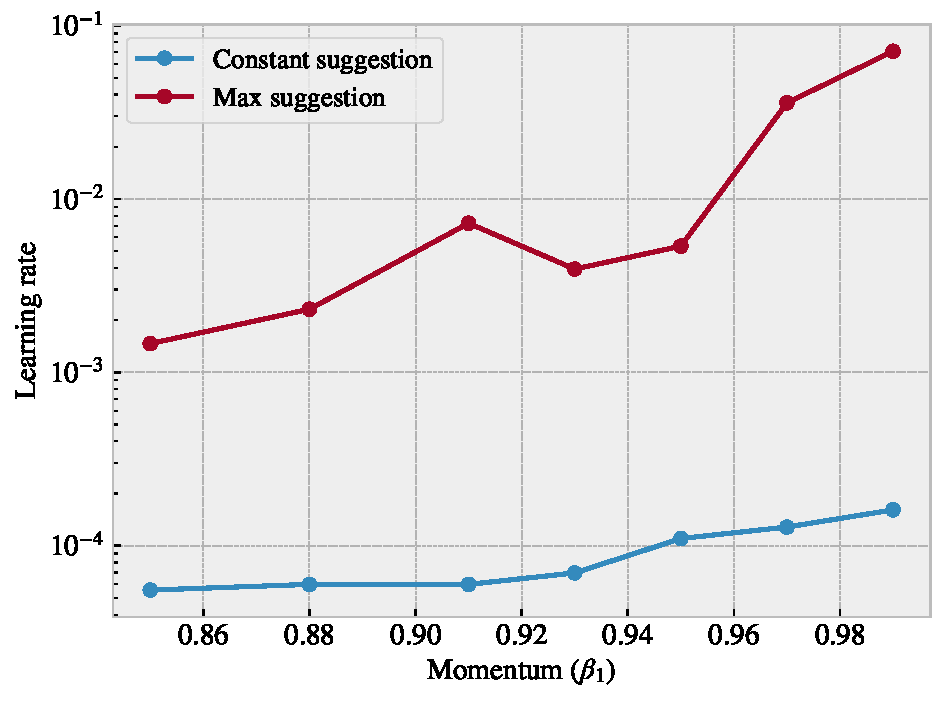
\includegraphics[width=\textwidth]{figures/ML/LR_momentum_test_b.pdf}
      \caption{}
      % \label{fig:}
  \end{subfigure}
  \hfill
  \caption{Momentum learning rate range tets}
  \label{fig:LR_range_mom}
\end{figure}


\begin{figure}[H]
  \centering
  \begin{subfigure}[t]{1.0\textwidth}
      \centering
      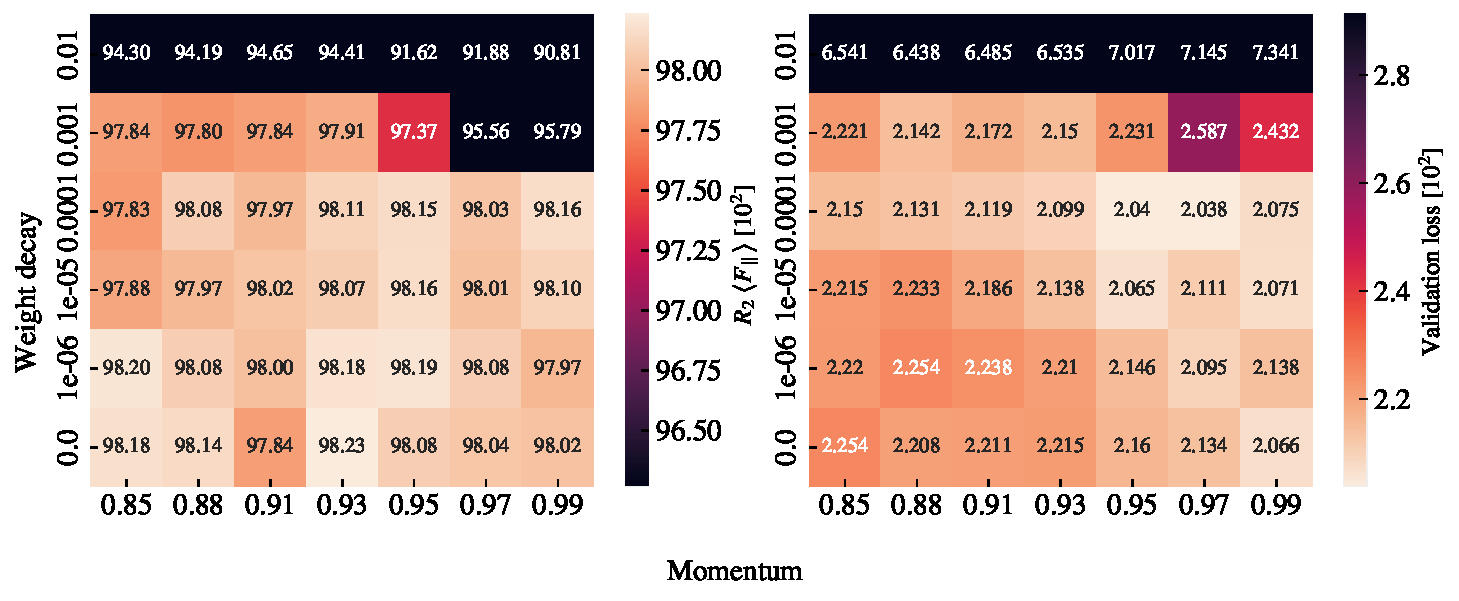
\includegraphics[width=\textwidth]{figures/ML/mom_weight_search_constant_perf.pdf}
      \caption{Validation performance.}
      % \label{fig:}
  \end{subfigure}
  \hfill
  \begin{subfigure}[t]{1.0\textwidth}
      \centering
      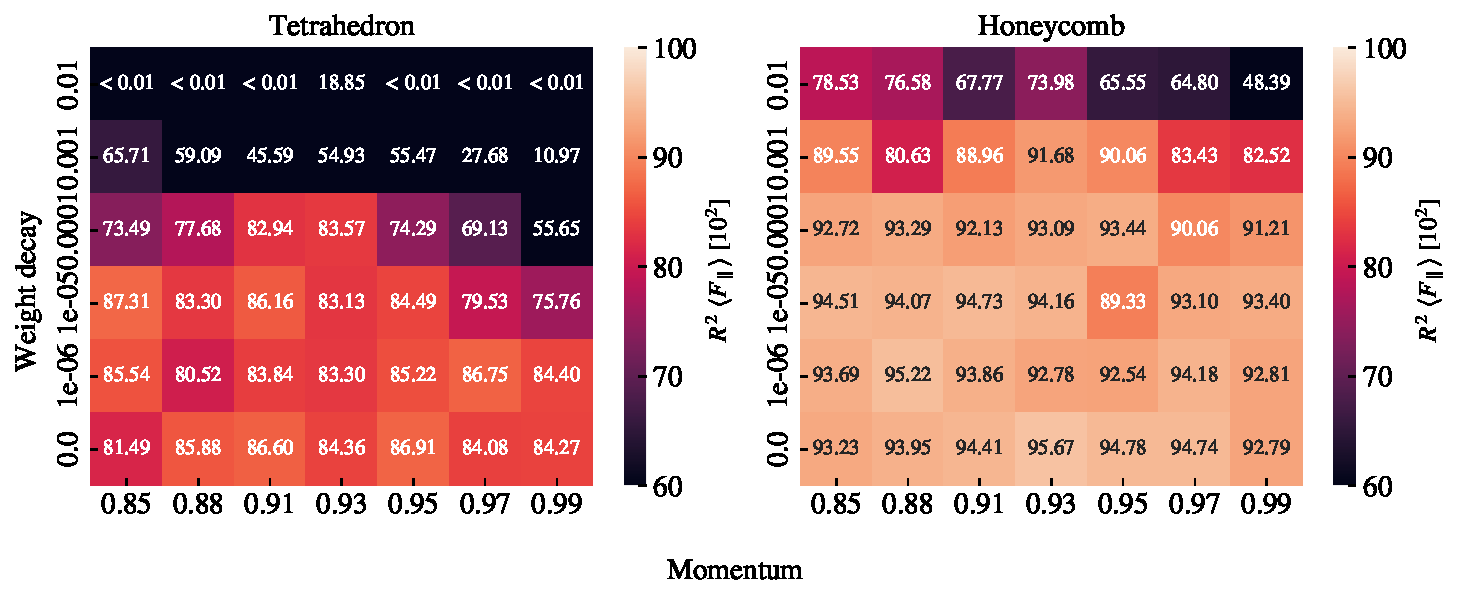
\includegraphics[width=\textwidth]{figures/ML/mom_weight_search_compare_constant_perf.pdf}
      \caption{Selected set comparison.}
      % \label{fig:}
  \end{subfigure}
  \hfill
  \caption{Constant learning rate and momentum scheme}
  \label{fig:mom_weight_search_constant}
\end{figure}

\begin{figure}[H]
  \centering
  \begin{subfigure}[t]{1.0\textwidth}
      \centering
      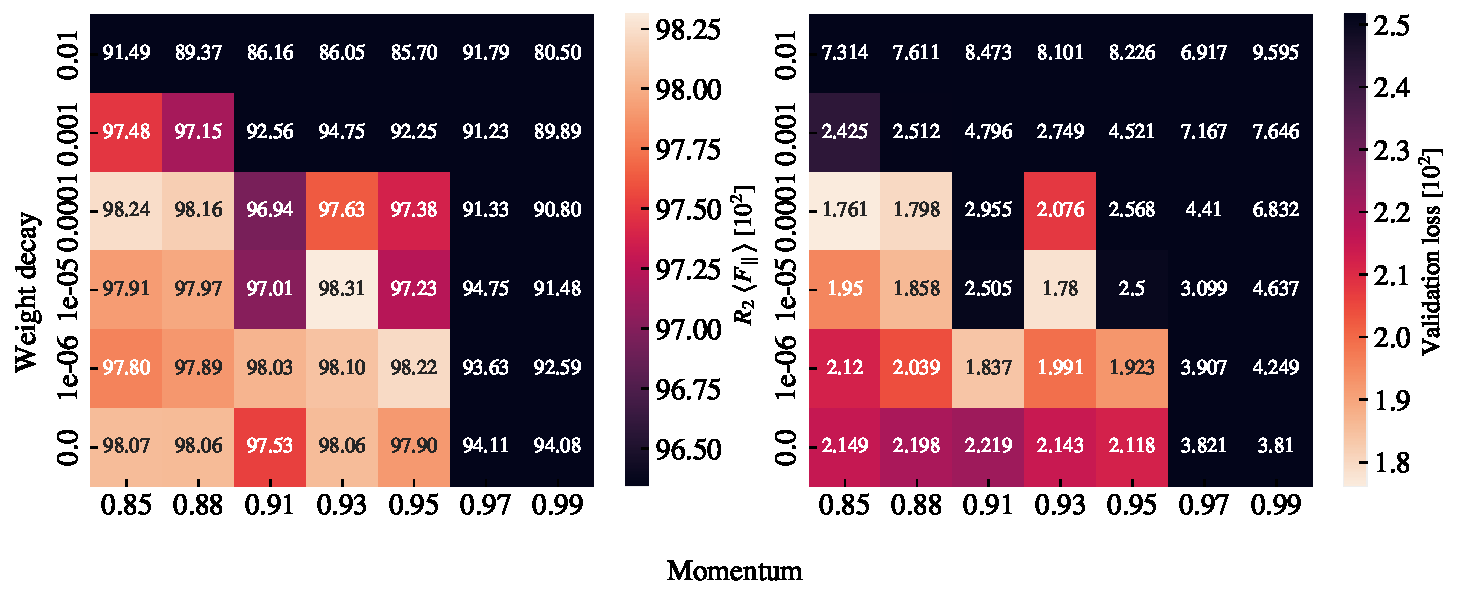
\includegraphics[width=\textwidth]{figures/ML/mom_weight_search_cyclic_perf.pdf}
      \caption{Validation performance.}
      % \label{fig:}
  \end{subfigure}
  \hfill
  \begin{subfigure}[t]{1.0\textwidth}
      \centering
      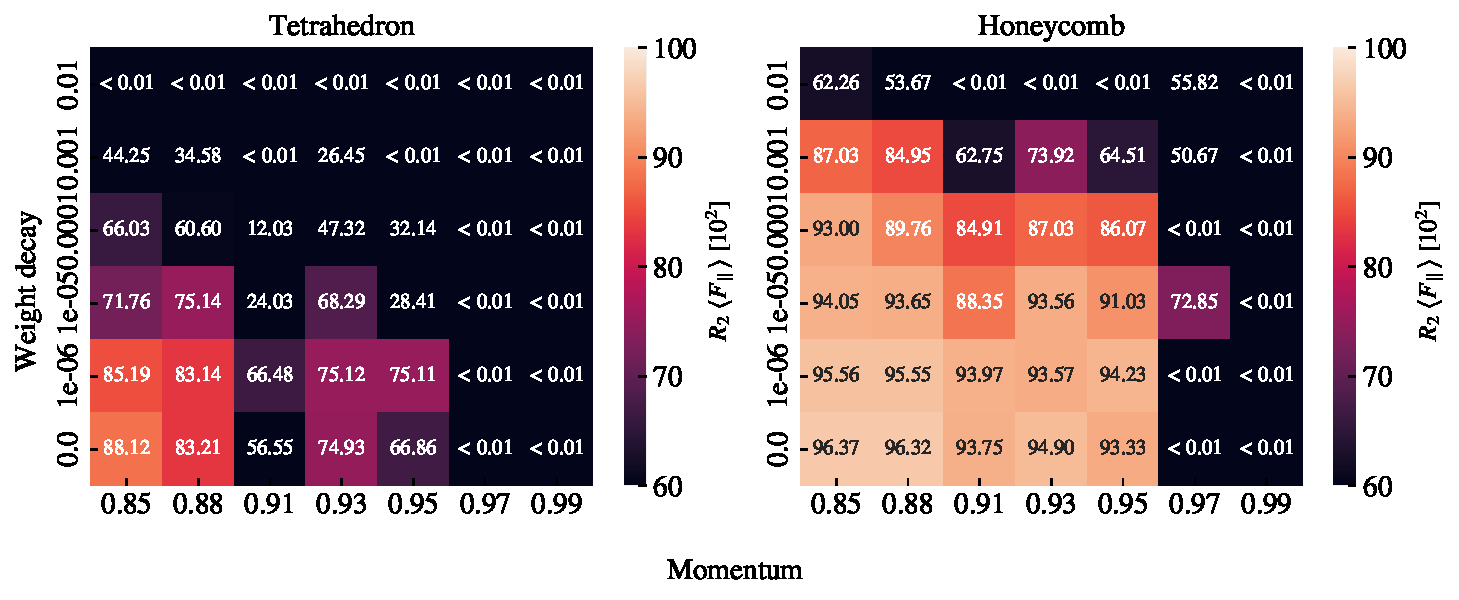
\includegraphics[width=\textwidth]{figures/ML/mom_weight_search_compare_cyclic_perf.pdf}
      \caption{Selected set comparison.}
      % \label{fig:}
  \end{subfigure}
  \hfill
  \caption{Cyclic learning rate and momentum scheme}
  \label{fig:mom_weight_search_cyclic}
\end{figure}


The original validation scores, before varying momentum and weight decay, were a
validation loss of 0.02124 and a mean friction $R_2$ score of 0.9816. By varying
momentum and weight decay, we can improve these scores slightly for the constant
learning rate scheme (loss: 0.02038, $R_2$: 0.9823) and even more for the cyclic
scheme (loss: 0.0176, $R_2$: 0.9831). However, these values are not taken from the same hyperparameter settings and we did not find a better option across all evaluation metrics. The comparison among best scores is
summarized in~\cref{tab:mom_weight_search}. In general, the constant scheme
shows rather stable results for all momentum settings $m \in [0.85, 0.99]$ in
combination with a low weight decay $\lambda \le \num{e-4}$. For the cyclic scheme
the performance peaks towards a low momentum $m \le 0.93$ and low weight decay
$\lambda \le \num{e-4}$. Looking at the summary in~\cref{tab:mom_weight_search} we
see that the cyclic scheme can produce a high score among all four
performance metrics, but since these scores do not share common hyperparameters we need to choose which of them to prioritize. Due to our interest in capturing the non-linear trends, we prioritize the score from the
selected set of Tetrahedron patterns as this provided the greatest challenge for our model to capture. We recognize that this choice introduces a greater risk of
overfitting since the data points within this evaluation set are partly included in the training set as well. This is especially alarming since the abscent of weight decay allow for more overfitting in general. However, for the purpose of performing an accelerated search, we find it more important to increase the chances of discovering novel designs than to reduce the chance of getting false positive results. Since we retain the option to verify the properties of a given design through \acrshort{MD} simulations afterward, we do not have to rely on the machine learning prediction as a final score. Thus we choose the cyclic trained model with low momentum $m = 0.85$ and zero weight decay as our final model. On a final note we also point out that our choice of hyperparameters corresponded to the edge of our grid search, and it would have been natural to perform an extended search in that range. This was omitted due to time prioritization and the belief that the potential gain of doing so was not huge.


\begin{table}[H]
  \begin{center}
  \caption{Momentum and weight decay grid search using S32D12 model.}
  \label{tab:mom_weight_search}
  \begin{tabular}{|c|c|c|c|c|} \hline
     &  & Score [\num{e2}] & Momentum & Weight decay \\ \hline
     \multirow{3}{*}{Validation loss} & Original & 2.124 & 0.9 & 0  \\ 
      & Constant & 2.038 & 0.97 & \num{e-4} \\ 
      & Cyclic & 1.761 & 0.85 & \num{e-4} \\ \hline
     \multirow{3}{*}{Validation $R_2$} & Original & 98.16 & 0.9 & 0  \\ 
      & Constant & 98.23 & 0.93 & 0 \\ 
      & Cyclic & 98.31 & 0.93 & \num{e-5} \\ \hline
     \multirow{3}{*}{Tetrahedron $R_2$} & Original & 87.07 & 0.9 & 0  \\ 
      & Constant & 87.31 & 0.85 & \num{e-5} \\ 
      & Cyclic & 88.12 & 0.85 & 0 \\ \hline
     \multirow{3}{*}{Honeycomb $R_2$} & Original & 94.78 & 0.9 & 0  \\ 
      & Constant & 95.67 & 0.93 & 0 \\ 
      & Cyclic & 96.37 & 0.85 & 0 \\ \hline
  \end{tabular}
  \end{center}
\end{table}

% ???
% Look at training history plots an show the overfitting (after best epoch)
% ???



\subsection{Final model}
From the hypertuning process, we choose the S32D12 model trained by a cyclic
training scheme with a momentum of 0.85, an accordingly chosen learning rate
from the learning range test and zero weight decay. The model contains
\num{1.3e7} model parameters. The main performance metrics are shown
in~\cref{tab:final_model_eval} where ``Tetrahedron'' and ``Honeycomb'' refer to
the selected set scores. Although we have mainly considered the mean friction
$R^2$ score during the hypertuning we find that the performance on the remaining
parameters is reasonable as well. The validation set reveals a final $R^2$ score
for the mean friction of $\sim 98 \%$ and a rupture accuracy of $\sim 96 \%$.
Since the data only contains roughly $12 \%$ ruptures this should be compared to
the accuracy score of $88 \%$ corresponding to never predicting a rupture.
Looking at the relative error for the rupture strain we find a large error of
$\sim 13 \%$. This is lower for the Tetrahedron ($5.9\%$) and Honeycomb
$(1.5\%)$ set. Thus we might get the idea that the relative error is especially
high on the validation set due to a few cases of very low rupture strains in the
Random walk patterns which would shift up the average.

\hl{I find it a bit disturbing to use the ``$\sim$'' too much, but I would like to indicate that a round the numbers... can I omit it?}

\cref{fig:final_model_eval} shows the mean friction, max friction and relative contact in comparison to the Tetrahedron $(7, 5, 1)$ and Honeycomb $(2,2,1,5)$ used in the pilot study. We note that these configurations are also partly contained within the training data, but this serves as a visualization of how the fit looks for $R^2$ scores above $98 \%$. We will evaluate a true test set later on based on the proposals from the accelerated search. 


\begin{table}[H]
  \begin{center}
  \caption{Mean values are used over different configurations.}
  \label{tab:final_model_eval}
  \begin{tabular}{ | c | c | c | c | c | c | c | c |} \hline
    & Loss [\num{e2}] & \multicolumn{3}{c|}{$R_2$ [\num{e2}]} & Abs. [\num{e2}] & Rel. [\num{e2}]  & Acc. [\num{e2}] \\ \hline
    & Total & Mean $F_f$ & Max $F_f$ & Contact & Porosity & Rup.\ Strain & Rupture \\ \hline
  Validation  & 2.1488 & 98.067 & 93.558 & 94.598 & 2.325 & 12.958 & 96.102 \\ \hline
  Tetrahedron & 4.0328 & 88.662 & 85.836 & 64.683 & 1.207 & \phantom{0}5.880 & 99.762 \\ \hline
  Honeycomb   & 8.6867 & 96.627 & 89.696 & 97.171 & 1.040 & \phantom{0}1.483 & 99.111 \\ \hline
  \end{tabular}
  \end{center}
\end{table}


\begin{figure}[H]
  \centering
  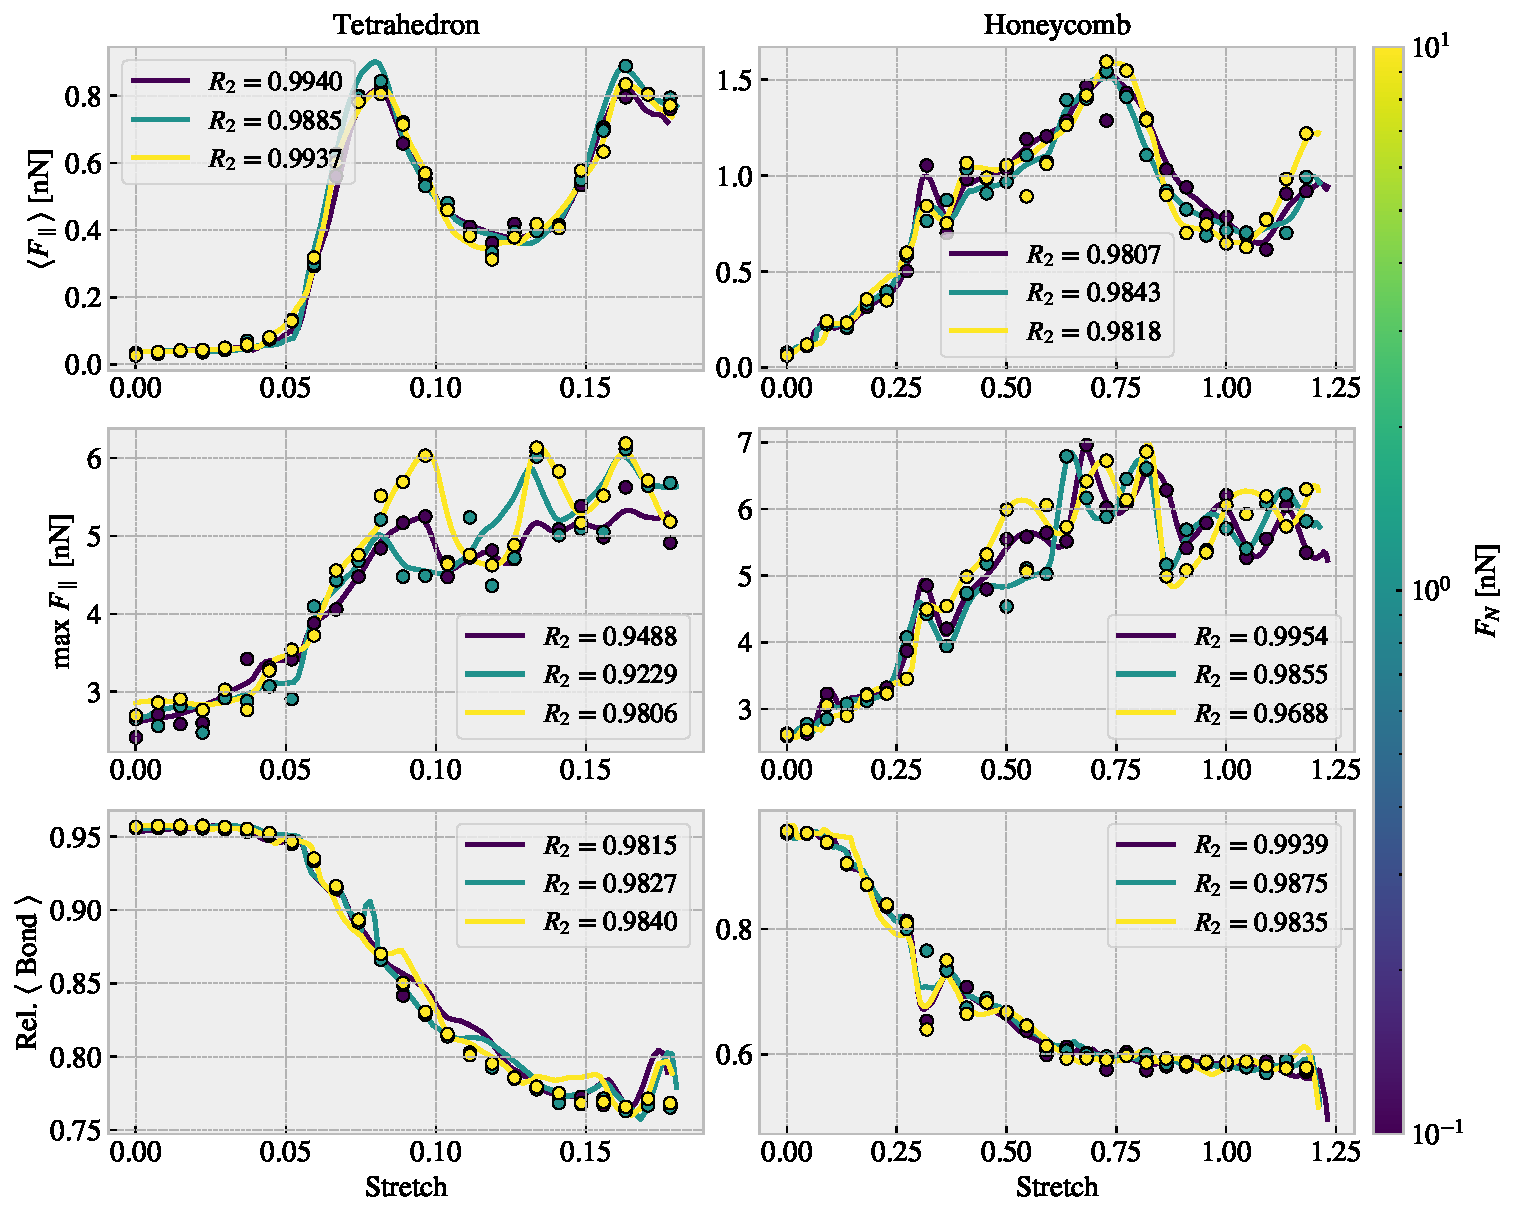
\includegraphics[width=\linewidth]{figures/ML/final_model_evaluation.pdf}
  \caption{With \num{e3} points in the strain range [0, 1.5] and stopping after first rupture prediction.}
  \label{fig:final_model_eval}
\end{figure}  

Using our final model, we evaluate the performance for the task of ranking the
configurations by the properties of interest. That is, we go through all the
configurations in the dataset, for the Tetrahedron, Honeycomb and Random walk
respectively, calculate the properties of interest and sort the configurations
accordingly. This is shown in~\crefrange{tab:ML_ranking_pop}{tab:ML_ranking_RW}
in comparison to the actual ranking in the dataset. Generally, we find that the
\acrshort{ML} performs rather well in the ranking of the maximum properties by
getting the right configurations into the top 3 three, while it is performing a
lot worse for the minimum friction property. This latter observation can be
attributed to the fact that the precision needed for an accurate ranking among
the minimum friction cases is a lot greater than for the remaining properties.
This is supported by the fact that the model predicts the Random walk 12
(\cref{tab:ML_ranking_RW}) to have negative mean friction, showing a lack of
precision. For the maximum categories, we find that the model gives a slightly
better ranking for the Tetrahedon and Honeycomb in comparison to the Random walk
patterns. When considering the actual predicted property scores for the maximum
properties we find that the model predictions are generally within a $\sim 0.2$
nN in the top 5. This gives an incentive that our model can be used to perform
an accelerated search of new configurations yielding a meaningful ranking of
property scores. 

% the task of assigning ordinal numbers, i.e.\ predicting the relative ranking, to the configurations. 

\begin{table}[H]
  \begin{center}
  \caption{Tetrahedon}
  \label{tab:ML_cranking_pop}
  \begin{tabular}{|c|c|c?{0.3mm}c|c|c|} \hline
    ML & \multicolumn{2}{c?{0.3mm}}{Data} &  \multicolumn{2}{c|}{\acrshort{ML}} & Data \\ \cline{2-5}
    Rank & Config & Value [nN] & Config & Value [nN] & Rank \\ \hline
    \multicolumn{6}{|c|}{$\min F_{\text{fric}}$} \\ \hline
    20 & (3, 9, 4) & 0.0067 & (3, 1, 2) & 0.0041 & 5  \\ \hline
    5 & (3, 1, 3) & 0.0075 & (1, 3, 4) & 0.0049 & 11 \\ \hline
    6 & (5, 3, 4) & 0.0084 & (1, 3, 3) & 0.0066 & 6  \\ \hline
    21 & (1, 7, 3) & 0.0084 & (3, 1, 4) & 0.0066 & 8  \\ \hline
    1 & (3, 1, 2) & 0.0097 & (3, 1, 3) & 0.0078 & 2  \\ \hline
    \multicolumn{6}{|c|}{$\max F_{\text{fric}}$} \\ \hline
    1 & (5, 3, 1) & 1.5875 & (5, 3, 1) & 1.5920 & 1 \\ \hline
    2 & (1, 3, 1) & 1.4310 & (1, 3, 1) & 1.2739 & 2 \\ \hline
    4 & (3, 1, 2) & 1.0988 & (9, 3, 1) & 1.1162 & 4 \\ \hline
    3 & (9, 3, 1) & 1.0936 & (3, 1, 2) & 0.7819 & 3 \\ \hline
    5 & (7, 5, 1) & 0.7916 & (7, 5, 1) & 0.7740 & 5 \\ \hline
    \multicolumn{6}{|c|}{$\max \Delta F_{\text{fric}}$} \\ \hline
    1 & (5, 3, 1) & 1.5529 & (5, 3, 1) & 1.5578 & 1 \\ \hline 
    2 & (1, 3, 1) & 1.3916 & (1, 3, 1) & 1.2331 & 2 \\ \hline 
    4 & (3, 1, 2) & 1.0891 & (9, 3, 1) & 1.0807 & 4 \\ \hline 
    3 & (9, 3, 1) & 1.0606 & (3, 1, 2) & 0.7778 & 3 \\ \hline 
    5 & (7, 5, 1) & 0.7536 & (7, 5, 1) & 0.7399 & 5 \\ \hline 
    \multicolumn{6}{|c|}{max drop} \\ \hline
    1 & (5, 3, 1) & 0.8841 & (5, 3, 1) & 0.8603 & 1 \\ \hline 
    2 & (3, 5, 1) & 0.4091 & (3, 5, 1) & 0.3722 & 2 \\ \hline 
    4 & (7, 5, 1) & 0.3775 & (1, 1, 1) & 0.2879 & 5 \\ \hline 
    5 & (9, 7, 1) & 0.2238 & (7, 5, 1) & 0.2478 & 3 \\ \hline 
    3 & (1, 1, 1) & 0.1347 & (9, 7, 1) & 0.1302 & 4 \\ \hline 
  \end{tabular}
  \end{center}
\end{table}

\begin{table}[H]
  \begin{center}
  \caption{Honeycomb}
  \label{tab:ML_ranking_hon}
  \begin{tabular}{|c|c|c?{0.3mm}c|c|c|} \hline
    ML & \multicolumn{2}{c?{0.3mm}}{Data} &  \multicolumn{2}{c|}{\acrshort{ML}} & Data \\ \cline{2-5}
    Rank & Config & Value [nN] & Config & Value [nN] & Rank \\ \hline
    \multicolumn{6}{|c|}{$\min F_{\text{fric}}$} \\ \hline
    1 & (2, 5, 1, 1) & 0.0177 & (2, 5, 1, 1) & 0.0113 & 1 \\ \hline 
    9 & (2, 4, 5, 1) & 0.0187 & (2, 5, 5, 3) & 0.0149 & 7 \\ \hline 
    7 & (2, 4, 1, 1) & 0.0212 & (2, 5, 5, 1) & 0.0182 & 4 \\ \hline 
    3 & (2, 5, 5, 1) & 0.0212 & (2, 5, 3, 1) & 0.0186 & 5 \\ \hline 
    4 & (2, 5, 3, 1) & 0.0226 & (2, 4, 1, 3) & 0.0198  & 15 \\ \hline 
    \multicolumn{6}{|c|}{$\max F_{\text{fric}}$} \\ \hline
    1 & (2, 1, 1, 1) & 2.8903 & (2, 1, 1, 1) & 2.9171 & 1 \\ \hline 
    2 & (2, 1, 5, 3) & 2.2824 & (2, 1, 5, 3) & 2.4004 & 2 \\ \hline 
    6 & (2, 1, 3, 1) & 2.0818 & (2, 1, 5, 1) & 2.1060 & 5 \\ \hline 
    4 & (2, 1, 3, 3) & 2.0313 & (2, 1, 3, 3) & 1.9458 & 4 \\ \hline 
    3 & (2, 1, 5, 1) & 2.0164 & (2, 4, 1, 1) & 1.9381 & 6 \\ \hline 
    \multicolumn{6}{|c|}{$\max \Delta F_{\text{fric}}$} \\ \hline
    1 & (2, 1, 5, 3) & 2.0234 & (2, 1, 5, 3) & 2.1675 & 1 \\ \hline 
    2 & (2, 1, 1, 1) & 1.9528 & (2, 1, 1, 1) & 2.0809 & 2 \\ \hline 
    3 & (2, 4, 1, 1) & 1.8184 & (2, 4, 1, 1) & 1.9157 & 3 \\ \hline 
    4 & (2, 1, 3, 3) & 1.7645 & (2, 1, 3, 3) & 1.6968 & 4 \\ \hline 
    5 & (2, 4, 1, 3) & 1.4614 & (2, 4, 1, 3) & 1.5612 & 5 \\ \hline 
    \multicolumn{6}{|c|}{max drop} \\ \hline
    1 & (2, 3, 3, 3) & 1.2785 & (2, 3, 3, 3) & 1.3642 & 1 \\ \hline 
    2 & (2, 1, 3, 1) & 1.1046 & (2, 1, 3, 1) & 0.9837 & 2 \\ \hline 
    3 & (2, 3, 3, 5) & 0.8947 & (2, 3, 3, 5) & 0.9803 & 3 \\ \hline 
    4 & (2, 1, 5, 3) & 0.8638 & (2, 1, 5, 3) & 0.9556 & 4 \\ \hline 
    13 & (2, 5, 1, 1) & 0.8468 & (2, 4, 5, 3) & 0.8999 & 8 \\ \hline 
  \end{tabular}
  \end{center}
\end{table}


\begin{table}[H]
  \begin{center}
  \caption{RW}
  \label{tab:ML_ranking_RW}
  \begin{tabular}{|c|c|c?{0.3mm}c|c|c|} \hline
    ML & \multicolumn{2}{c?{0.3mm}}{Data} &  \multicolumn{2}{c|}{\acrshort{ML}} & Data \\ \cline{2-5}
    Rank & Config & Value [nN] & Config & Value [nN] & Rank \\ \hline
    \multicolumn{6}{|c|}{$\min F_{\text{fric}}$} \\ \hline
    1 & 12 & 0.0024 & 12 & -0.0011 & 1 \\ \hline 
    24 & 76 & 0.0040 & 06 & 0.0036  & 27 \\ \hline 
    6 & 13 & 0.0055 & 14 & 0.0074  & 23 \\ \hline 
    31 & 08 & 0.0065 & 05 & 0.0082  & 19 \\ \hline 
    26 & 07 & 0.0069 & 63 & 0.0085  & 57 \\ \hline 
    \multicolumn{6}{|c|}{$\max F_{\text{fric}}$} \\ \hline
    3 & 96 & 0.5758 & 99 & 0.5155 & 2 \\ \hline 
    1 & 99 & 0.5316 & 98 & 0.4708 & 3 \\ \hline 
    2 & 98 & 0.4478 & 96 & 0.4356 & 1 \\ \hline 
    4 & 97 & 0.3624 & 97 & 0.3503 & 4 \\ \hline 
    11 & 58 & 0.3410 & 55 & 0.2817 & 7 \\ \hline 
    \multicolumn{6}{|c|}{$\max \Delta F_{\text{fric}}$} \\ \hline
    3 & 96 & 0.5448 & 99 & 0.4669 & 2 \\ \hline 
    1 & 99 & 0.4769 & 98 & 0.4314 & 3 \\ \hline 
    2 & 98 & 0.4085 & 96 & 0.4128 & 1 \\ \hline 
    4 & 97 & 0.3268 & 97 & 0.3080 & 4 \\ \hline 
    78 & 57 & 0.2978 & 55 & 0.2542 & 7 \\ \hline 
    \multicolumn{6}{|c|}{max drop} \\ \hline
    3 & 01 & 0.1818 & 00 & 0.1883 & 3 \\ \hline 
    2 & 96 & 0.1733 & 96 & 0.1654 & 2 \\ \hline 
    1 & 00 & 0.1590 & 01 & 0.1532 & 1 \\ \hline 
    11 & 37 & 0.1022 & 04 & 0.0591 & 8 \\ \hline 
    28 & 34 & 0.0879 & 56 & 0.0552 & 20 \\ \hline 
  \end{tabular}
  \end{center}
\end{table}


\section{Accelerated Search}
From~\cref{eq:ML} we have found promising results that we can use a machine learning model to predict the friction behavior. This enables us to omit the \acrshort{MD} simulations in the evaluation process and perform an accelerated search through new configurations. We will use the friction properties of interest as our main optimization metrics. We approach the accelerated search by two different methods:
\begin{enumerate}
  \item Using the generative algorithms developed for the creation of the Tetrahedron, Honeycomb and Random walk patterns, we create an extended dataset and evaluate the performance using the \acrshort{ML} model.
  \item Using the genetic algorithm method we perturb (mutate) the configurations and optimize for the maximum drop property using the \acrshort{ML} model to evaluate the fitness function. 
\end{enumerate}


\subsection{Patteren generation search}
We utilize the pattern generators developed in~\cref{chap:system} to create an extended dataset for our search. For the Tetrahedron and Honeycomb patterns, the increment of the parameters will lead to an increased spacing within the pattern. This will eventually lead to the main pattern structures exceeding the size of the sheet. Thus, we can essentially perform a full search ``maxing out'' the parameters of these patterns. We estimate
that this is done with the max parameters, $(60, 60, 30)$ for the Tetrahedron,
and $([30, 30, 30, 60])$ for the Honeycomb pattern. We use a random reference position
and regenerate each unique parameter 10 times to explore translational effects. This gives in total 135k configurations for the
Tetrahedron pattern and 2025k for the Honeycomb pattern. For the Random walk
generator, we do a Monte Carlo sampling. In each sample, we draw the scalar values, either from a uniform (U) or logarithmic uniform (LU) distribution as follows.
\begin{align*}
  \text{Num. walks} &\sim \text{U}[1, 30] & \text{Max. steps} &\sim \text{U}[1,30]  & \text{Min. dis.} &\sim \text{U}[0,4] \\
  \text{Bias direction} &\sim \text{U}[0, 2\pi] & \text{Bias. strength} &\sim \text{LU}[0,10]  & p_{\text{stay}} &\sim \text{U}[0,1]  
\end{align*}
Notice that we use discrete distribution for the parameters requiring integers.
For the binary parameters \textit{Connection}, \textit{Avoid invalid},
\textit{RN6} and \textit{Grid start} we simply set the values by a 50--50
chance. The remaining parameters are kept constant at \textit{Periodic: True}
and \textit{Centering: False} throughout the search. For the handling of
clustering, we implement the repair algorithm such that the sheet is repaired by
the least modifications approach rather than retrying the generation several
times \hl{Make sure that this is introduced somewhere}. Due to the extra
computation time associated with the random walk and the repair algorithm, we
only generate 10k configurations within this class. For the \acrshort{ML}
evaluation of the configurations we use a normal load of \SI{5}{nN} and generate
a strain curve in the domain $[0,2]$ using 100 evenly spaced points. We compute
the properties of interest and rank the configurations accordingly. The top
candidates for each property are shown in~\cref{tab:pattern_search} including a
comparison to the original dataset top candidates
from~\cref{tab:data_properties}. The random walk top five candidates are
visualized in~\cref{fig:RW_search_top5}.


\begin{table}[H]
  \begin{center}
  \caption{Pattern search. The values are in units nN.}
  \label{tab:pattern_search}
  \begin{tabular}{|L{1.75cm} |c|c|c| c |c|c|c|} \cline{2-4} \cline{6-8}
  \multicolumn{1}{c|}{} & \multicolumn{3}{c|}{Search}  && \multicolumn{3}{c|}{Data} \\ \cline{2-4} \cline{6-8}
  \multicolumn{1}{c|}{\textbf{Scores}} & Tetrahedron & Honeycomb & Random walk && Tetrahedron & Honeycomb & Random walk \\ \cline{1-4} \cline{6-8}
  $\min F_{\text{fric}}$         & $-0.062 \ \ $  & $-0.109 \ \ $  & $-0.061 \ \ $ &&   0.0067 & 0.0177 & 0.0024 \\ \cline{1-4} \cline{6-8}
  $\max F_{\text{fric}}$         & $1.089$        & $2.917$        & $0.660$       &&   1.5875 & 2.8903 & 0.5758 \\ \cline{1-4} \cline{6-8}
  $\max \Delta F_{\text{fric}}$  & $1.062$        & $2.081$        & $0.629$       &&   1.5529 & 2.0234 & 0.5448 \\ \cline{1-4} \cline{6-8}   
  max drop                      & $0.277$        & $1.250$        & $0.269$       &&   0.8841 & 1.2785 & 0.1818 \\ \cline{1-4} \cline{6-8}   
  \multicolumn{8}{c|}{} \\ \cline{2-4} \cline{6-8}
  \multicolumn{1}{c|}{\textbf{Configs.}} & Tetrahedron & Honeycomb & Random walk  && Tetrahedron & Honeycomb & Random walk  \\ \cline{1-4} \cline{6-8}
  $\min F_{\text{fric}}$         & $(13,11,14)$ & $(14,25,7,19)$  & \textit{no name} &&   $(3,9,4)$ & $(2,5,1,1)$ & 12 \\ \cline{1-4} \cline{6-8}
  $\max F_{\text{fric}}$         & $(1,3,1)$    & $(2,1,1,1)$     & \textit{no name} &&   $(5,3,1)$ & $(2,1,1,1)$ & 96 \\ \cline{1-4} \cline{6-8}
  $\max \Delta F_{\text{fric}}$  & $(1,3,1)$    & $(2,1,1,1)$     & \textit{no name} &&   $(5,3,1)$ & $(2,1,5,3)$ & 96 \\ \cline{1-4} \cline{6-8}   
  max drop                      & $(1,7,1)$    & $(3,3,5,3)$     & \textit{no name} &&   $(5,3,1)$ & $(2,3,3,3)$ & 01 \\ \cline{1-4} \cline{6-8}   
  \end{tabular}
  \end{center}
\end{table}

First of all, we notice that the top candidates for the minimum friction are all
predicted to have a negative friction value. This unphysical prediction aligns with the previous observations that our model does not have the required precision to yield accurate predictions for this property. Moreover, we can argue that pursuing the optimization for a low friction value will eventually highlight the weaknesses of the model as we reward an unphysical negative value. In order to resolve this problem one might need to extend the training dataset and possibly include a physical constraint for positive friction values. However, by consulting the proposed minimum candidates we find that they all share the same feature of being sparsely cut.
For the Random walk, we see this visually in~\cref{fig:RW_search_top5}, while
for the Tetrahedon and Honeycomb patterns, this is evident from the
configuration parameters shown in~\cref{tab:pattern_search} where the parameters
reveal a high spacing between the cuts. The porosity of the minimum friction top
candidates are all rather low being $1.5\%$, $5.6\%$, and $1.6\%$ for the
Tetrahedron, Honeycomb and Random walk respectively. This further supports the idea that the Kirigami sheet can not readily be used to reduce friction within our system domain since the results point toward a non-cut sheet as the best minimum friction candidate.


\begin{figure}[H]
  \centering
  \includegraphics[width=\linewidth]{figures/search/RW_search_top5.pdf}
  \caption{RW search top results.}
  \label{fig:RW_search_top5}
\end{figure}  


Among the remaining maximum properties, we find competing values for the
Honeycomb and Random walk classes. However, the top-scoring values for the Honeycomb correspond to configurations within the original dataset which is also the case for the Tetrahedron top candidates. The only difference is the randomized reference position. When taking a closer look at the ranking for
each property it becomes apparent that the predictions are highly sensitive to
the reference position parameter used for the Tetrahedron and Honeycomb
pattern. Since we repeated each pattern parameter 10 times with a random reference
position, we initially expected to get a ranking in sets of 10. However, the
ranking only shows contiguous appearing sets in the range of 1--5 which points toward a dependency on pattern translation. Hence we investigate this further by
evaluating the scores for a systematic change of the reference position. We generally find the max drop parameter to give the
highest variation and thus we show the max drop scores for the max drop top candidates Tetrahedron $(1,7,1)$, $(5,3,1)$ and Honeycomb $(3,3,5,3)$, $(2,3,3,3)$ in~\cref{fig:ref_search_top_data}. The results show that the max drop property prediction varies drastically with the translation of these patterns. The emerging question is
then whether this is grounded in a physical phenomenon or simply a
deficiency in the \acrshort{ML}. Even though the patterns are periodic in the
x-y-plane, with a period according to the unique number of translations shown in~\cref{fig:ref_search_top_data}, the translation will determine the specific
configuration of the edge. Previous studies of static friction and stick-slip
behavior point to the importance of edge effects \hl{refer to theory or directly to the sources?}, and thus for a sheet where the atoms on the $\pm x$ free
edge constitute about 2.5\% of the inner sheet atom count, it is not
unreasonable that the translation might result in a significantly different
outcome. In that case, the search through reference positions highlights that
the translation can be key to optimizing for certain properties. However, the
results might also indicate that the model is either overfitted or that we
simply did not provide enough data to reach a generalization of the complex
physical behavior of the system. The sensible way forward to unravel this would
be to generate additional translational variants of the same configurations to
investigate for any physical edge dependencies or otherwise strengthen the
model by this data. We earmark this suggestion for another study. When considering some of the friction-strain curves we also find that the prediction of the rupture point plays an important role for the max drop property. As the rupture is often predicted on a descending part of the curve any variation to the rupture strain will affect the max drop property quite significantly.


\begin{figure}[H]
  \centering
  \begin{subfigure}[t]{0.49\textwidth}
      \centering
      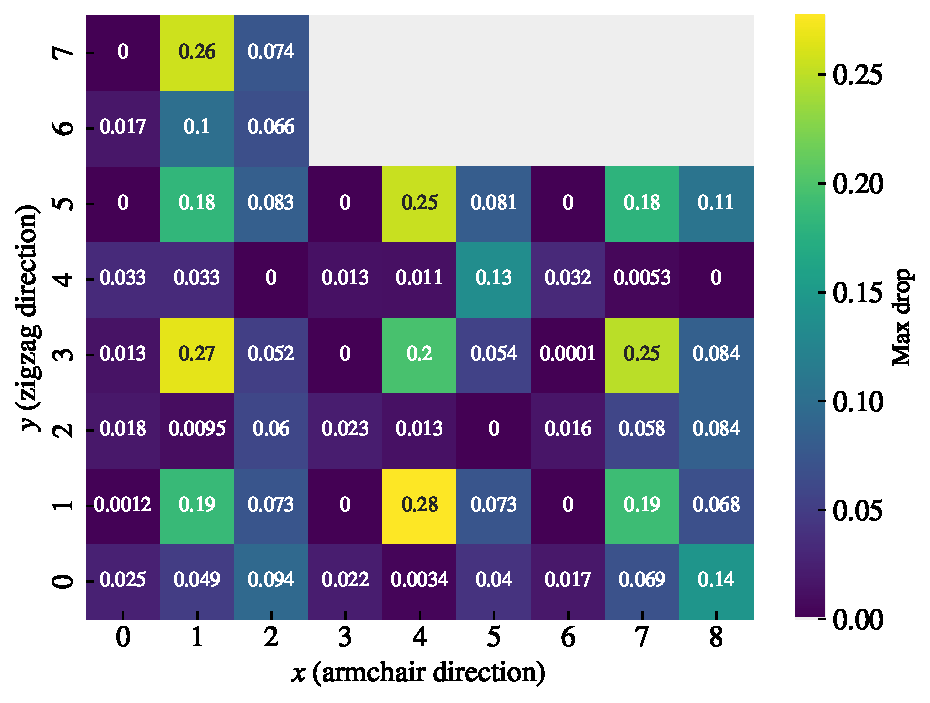
\includegraphics[width=\textwidth]{figures/search/ref_search_drop_pop_1_7_1_ref_search.pdf}
      \caption{Tetrahedron $(1,7,1)$ (60). Std = 0.08, Rel.\ Std = 1.13}
      % \label{fig:}
  \end{subfigure}
  \hfill
  \begin{subfigure}[t]{0.49\textwidth}
    \centering
    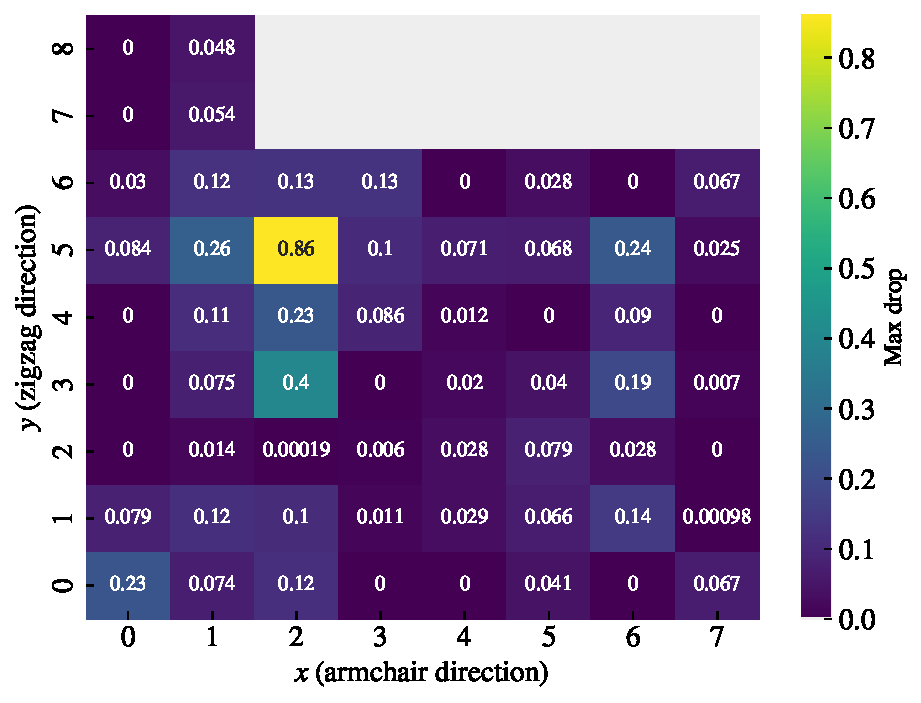
\includegraphics[width=\textwidth]{figures/search/ref_search_drop_pop_5_3_1_ref_search.pdf}
    \caption{Tetrahedron $(5,3,1)$ (60). Std = 0.13, Rel.\ Std = 1.61}
    % \label{fig:}
  \end{subfigure}
  \hfill
  \begin{subfigure}[t]{0.49\textwidth}
      \centering
      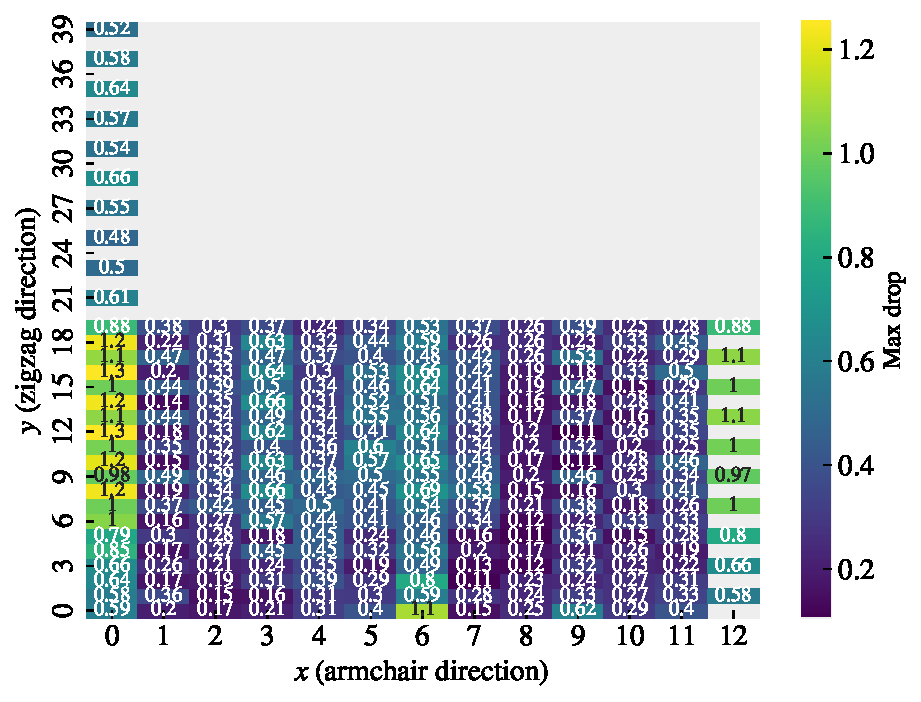
\includegraphics[width=\textwidth]{figures/search/ref_search_drop_hon_3_3_5_3_ref_search.pdf}
      \caption{Honeycomb $(3,3,5,3)$ (260). Std = 0.25, Rel.\ Std = 0.58}
      % \label{fig:}
  \end{subfigure}
  \hfill
  \begin{subfigure}[t]{0.49\textwidth}
      \centering
      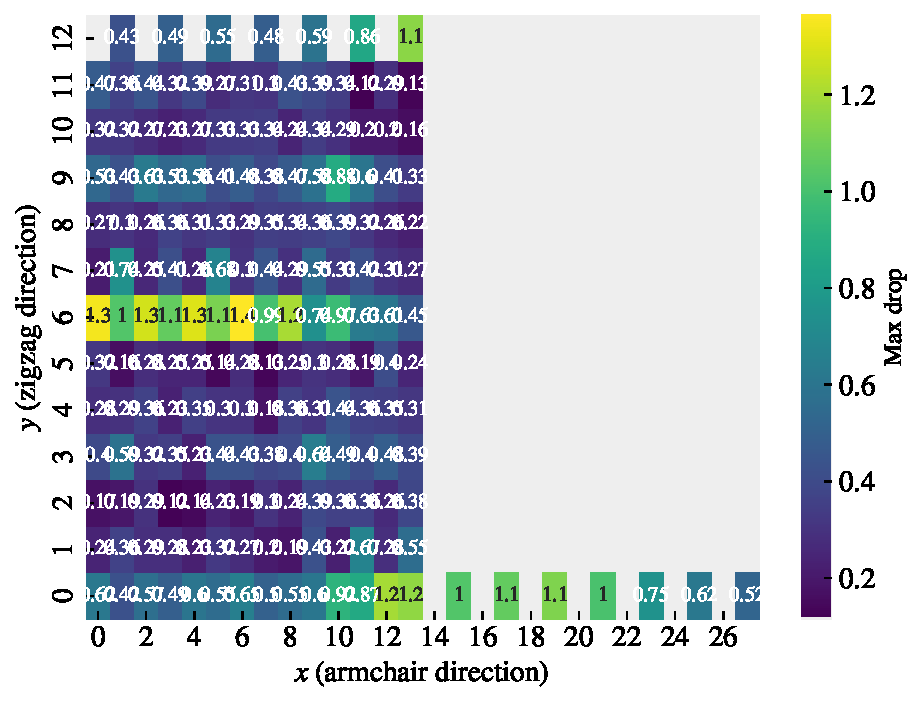
\includegraphics[width=\textwidth]{figures/search/ref_search_drop_hon_2_3_3_3_ref_search.pdf}
      \caption{Honeycomb $(2,3,3,3)$. (182)  Std = 0.27, Rel.\ Std = 0.60}
      % \label{fig:}
  \end{subfigure}
  \hfill
  \caption{\hl{CAPTION} \hl{Fix overlapping annotation text}}
  \label{fig:ref_search_top_data}
\end{figure}

In order to get insight into the generalization of the model, we
evaluate the performance on a true test set. We use the 20 configurations given by the top 5 candidates for each of the properties of interest in the Random walk search shown in n~\cref{fig:RW_search_top5}. We calculate the ground truth using \acrshort{MD} simulation by sampling 30 pseudo uniform strain values using a normal load of \SI{5}{nN}. Unfortunately, the test set reveals a significantly worse performance than the validation scores reported so far. It shows a loss
of 2.13, which is two orders of magnitude higher than the validation scores, an
average absolute error for the mean friction of \SI{0.14}{nN} and a rupture
accuracy of 70 \%. The mean friction average $R^2$ score is negative which indicates that our model performs worse than simply guessing on a constant
value given by the true data mean. This reveals that our model is not
generalized enough to provide accurate predictions on the newly generated Random
walk configurations. This can mainly be attributed two reasons: 1) The test set data distribution is not similar to that of the training and validation data drawn from the original data set. 2) The considerations of the selected Tetrahedron and Honeycomb dataset, which overlapped with the training data, has led to an overfitting of the model. However, by going back to the hypertuning process and choosing the best model (C16D8) from the architecture complexity grid test given by the lowest validation score, trained with a constant learning rate, we get similar
results. This indicates that the poor test result is not simply caused by the hypertuning choices. Instead, it points to the fact that our original training data does not contain a generalized distribution that accurately captures the full complexity of our system. This aligns with the high fluctuation in prediction value when translating the patterns. Thus we conclude that a machine learning approach might be feasible, given the promising validation scores, but that we need a bigger and more generalized dataset for a reliable prediction of new configurations. 






\subsection{Genetic algorithm search}
Despite the fact that our machine learning analysis indicates that the model is not generalized enough for an accurate prediction on new configurations, we investigate the prospects of using a genetic algorithm based accelerated search. So far we have concluded that a minimization of the friction is not
promising, and hence we discard this property for further study. We have also
seen that the maximum style properties often share similar top candidates, and
thus we choose to only investigate the max drop property, associated with the
aim of creating a negative friction coefficient. We verify our implementation of the genetic algorithm by optimizing a smaller $10 \times 10$ lattice for the maximum energy of the the Ising model without any external field. That is, we consider the Hamiltonian 
\begin{align*}
  H = -J\sum_{\langle kl \rangle} s_k s_l,
\end{align*}
for the square lattice sites $s$ with the sum running over nearest neighbouring sites $k$ and $l$. The sites take a binary value, either $-1$ or $+1$, and thus the highest energy for the system is reached for a checkboard pattern of every other side is $-1$ and the remaining being $+1$. We find that the algorithm converges toward the optimal solution within a hundred generations most of the time, which shows that it can handle some spatial dependencies in the matrix.

For the genetic algorithm search we use the top candidates from the pattern generation search as a starting point for the populations. That is, we generate the population based on the parameter associated with the max drop top candidates for the Tetrahedron, Honeycomb and Random walk search respectively. We generate a population of 100 configurations and run the search for  50 generations as we did not see much improvement for longer runs. The Tetrahedron and Honeycomb search did immediately give any useful results as the highest scoring individual from the population was not improved throughout the search even though the average score was rising initially. For the Random walk performed 5 runs based on the top 5 candidates. Most of them gave a similar result as seen for the Tetrahedon and
Honeycomb patterns with only a single run providing a new generated candidate. The score of this candidate was \SI{0.240}{nN} which is only a small improvement from the otherwise best Random walk max drop score of
\SI{0.182}{nN}. However, from the other non-improving runs the initialization of the Random walk based population provided a top score of \SI{0.345}{nN} which shows that we have better hopes of optimizing this property by simply generating more configurations from these parameters. 

The fact that starting from an existing design did not give any useful results, we attempt to start from a population of random noise as well. We initialize one population with mixed porosities, having 20 individuals each for porosity $\{0.01, 0.05, 0.1, 0.2, 0.3\}$, and two populations based on a porosity of 0.25 and 0.5
respectively. This time the algorithm improved the top candidate throughout, but
the final top scores are still not impressive. The mixed porosity start gave the
highest score, being \SI{0.299}{nN}. When considering the corresponding patterns of the top five candidates in this search, they were all visually quite
similar to the starting configurations; they still looked like random noise.
Thus, we do not find any significant signs that the genetic algorithm search can generate any higher-level pattern structures worth further investigating. This is of course likely to be connected with the fact that the machine learning model governing the fitness evaluation is unstable outside orignal data domain.


By the use of the Grad-CAM method, we examine some of the proposed patterns for
any noticeable trends in the model predictions. The result for the mixed
porosity search top candidate is shown in  ~\cref{fig:GC_mixed_p}. For
comparison, we included a similar examination for the top candidates in the
pattern generation search with respect to the max drop category for the
Tetrahedron, Honeycomb and Random walk, shown in
\crefrange{fig:GC_pop_search}{fig:GC_hon_search}. For the mixed porosity top
candidate, the Grad-CAM method highlights some areas in the noise configuration
as contributing more positively than others, but we do not find any obvious
trends from this. For the more structured patterns of the Tetrahedron, Honeycomb
and Random walk configurations we see in many cases throughout the straining
that cuts in the sheet are highlighted. This gives some confidence to the idea
that the model does consider some of the relevant features in the pattern, but
it still varies too much to make any strong conclusion. However, we notice that
for certain strain values, the Grad-CAM reveals considerable ``attention'' towards the edge of the configuration. This especially relates to the top and bottom edge ($\pm y$). For instance, \cref{fig:GC_hon_search} shows a highlighting of the bottom edge at strain 0.396 for the Honeycomb pattern. Considering that the top and bottom of the configuration are not a true edge, since these are connected to the pull blocks in the simulation, this is a bit surprising. One interpretation is that the dissipation associated with the thermostat in the pull blocks might be of importance. Even though, that these results should be taken carefully due to the instability of the model, we note this as a topic for further investigations. 



\begin{figure}[H]
  \centering
  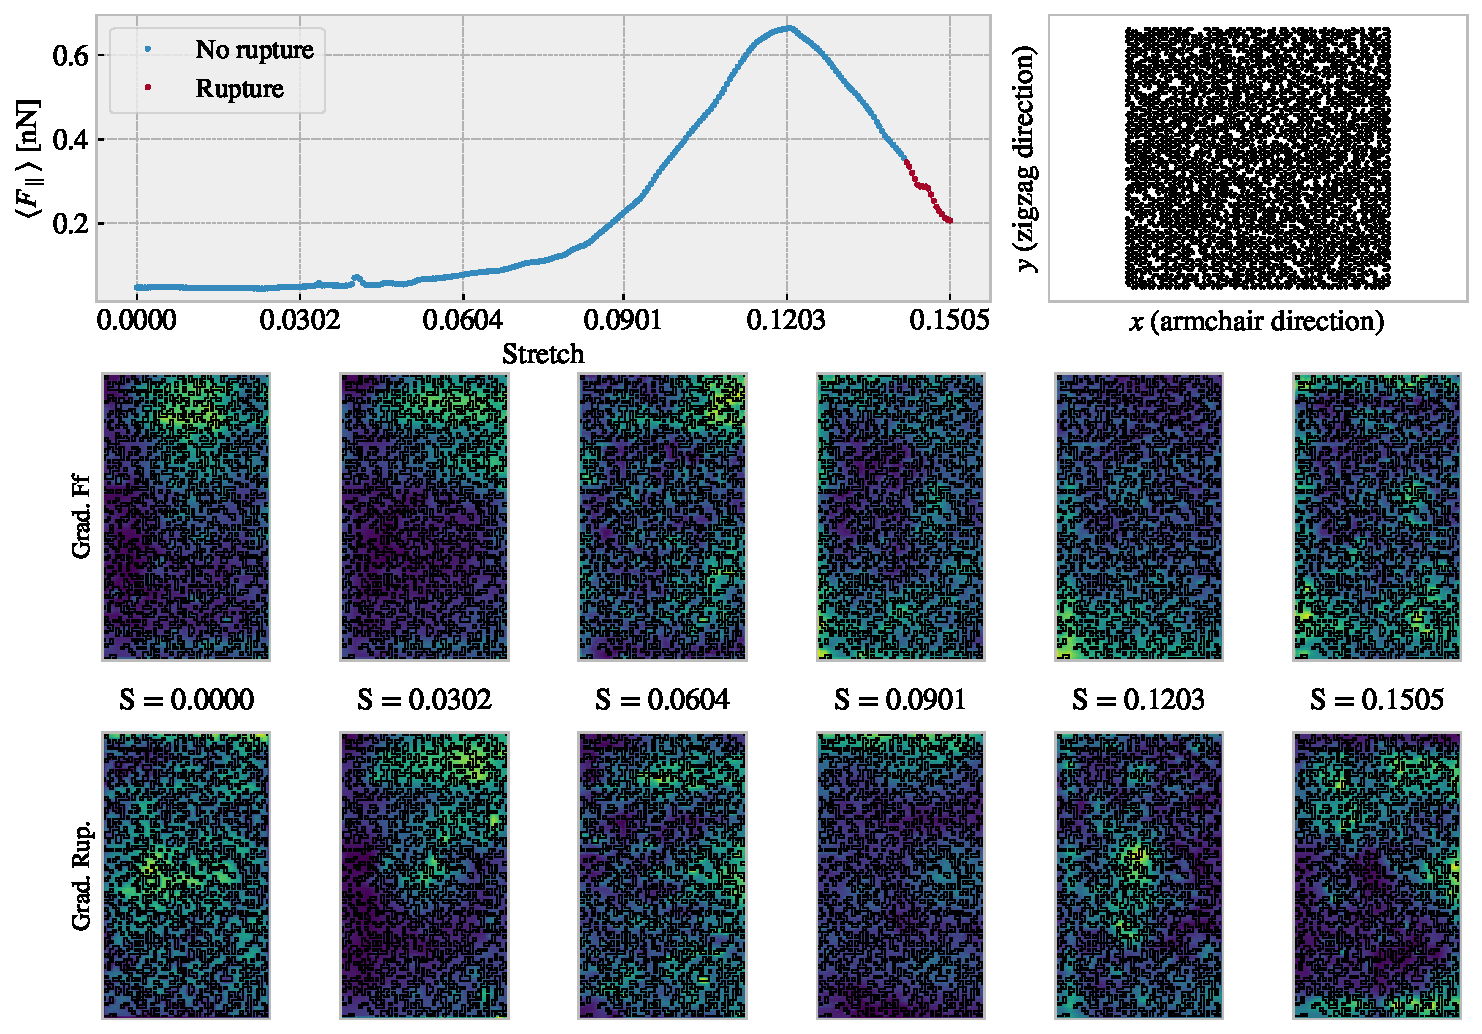
\includegraphics[width=0.8\linewidth]{figures/search/grad_cam_GA_RN_start_top0.pdf}
  \caption{$p \in \{0.01, 0.05, 0.1, 0.2, 0.3\}$.}
  \label{fig:GC_mixed_p}
\end{figure}  

\begin{figure}[H]
  \centering
  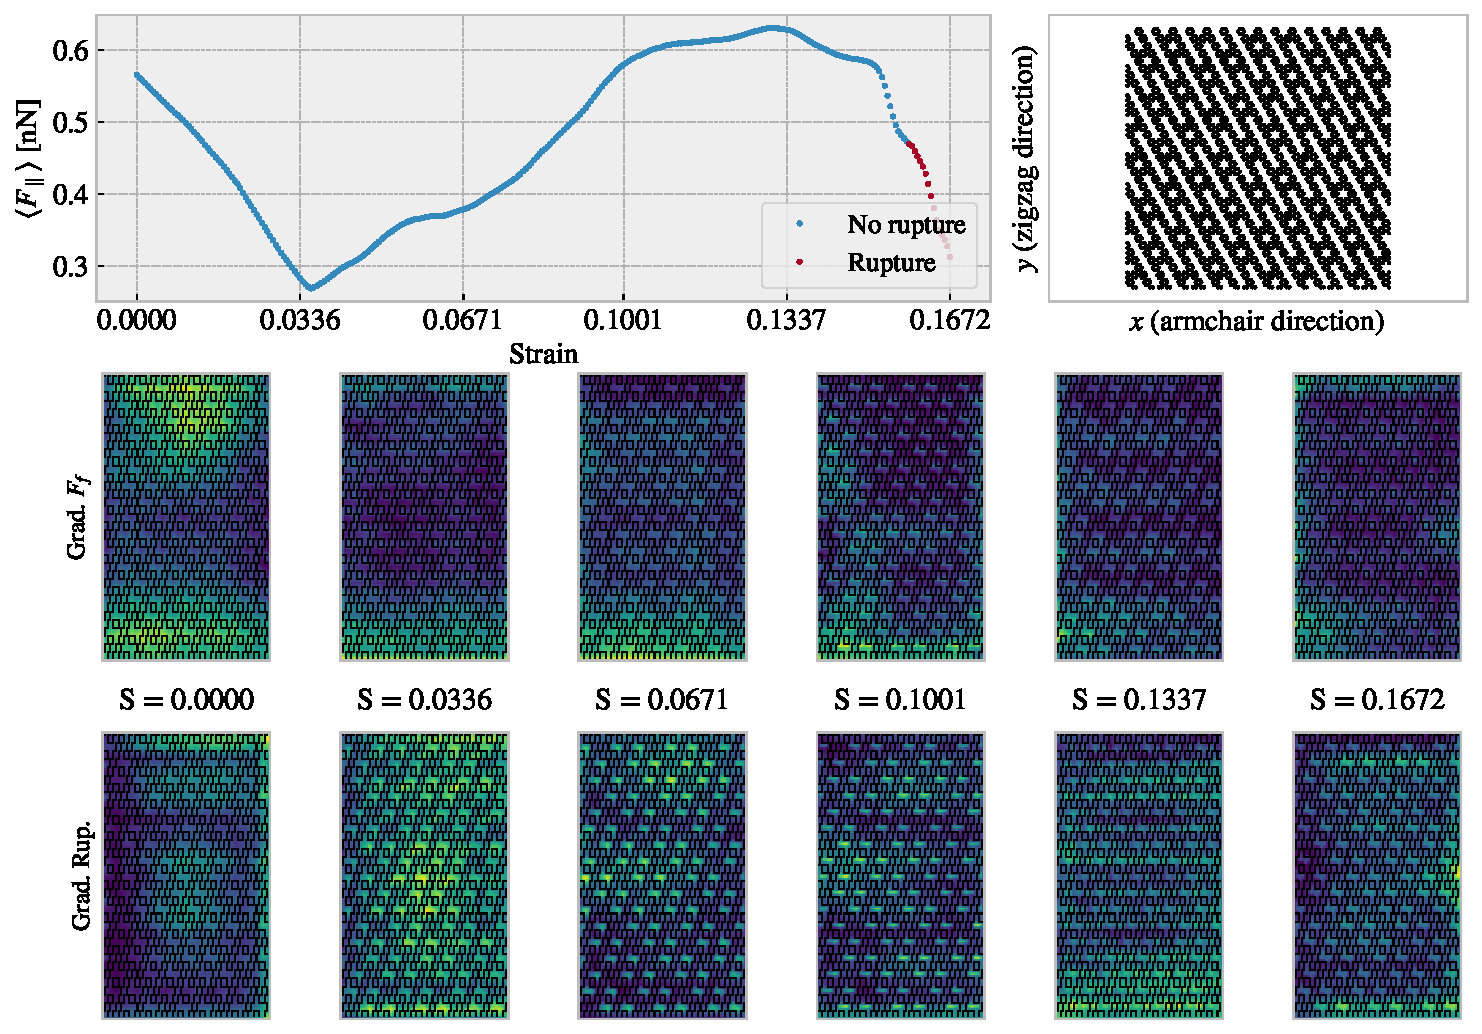
\includegraphics[width=0.8\linewidth]{figures/search/grad_cam_pop_1_7_1_1_4.pdf}
  \caption{Tetrahedron $(1,7,1)$, ref = $(1,4)$}
  \label{fig:GC_pop_search}
\end{figure}  


\begin{figure}[H]
  \centering
  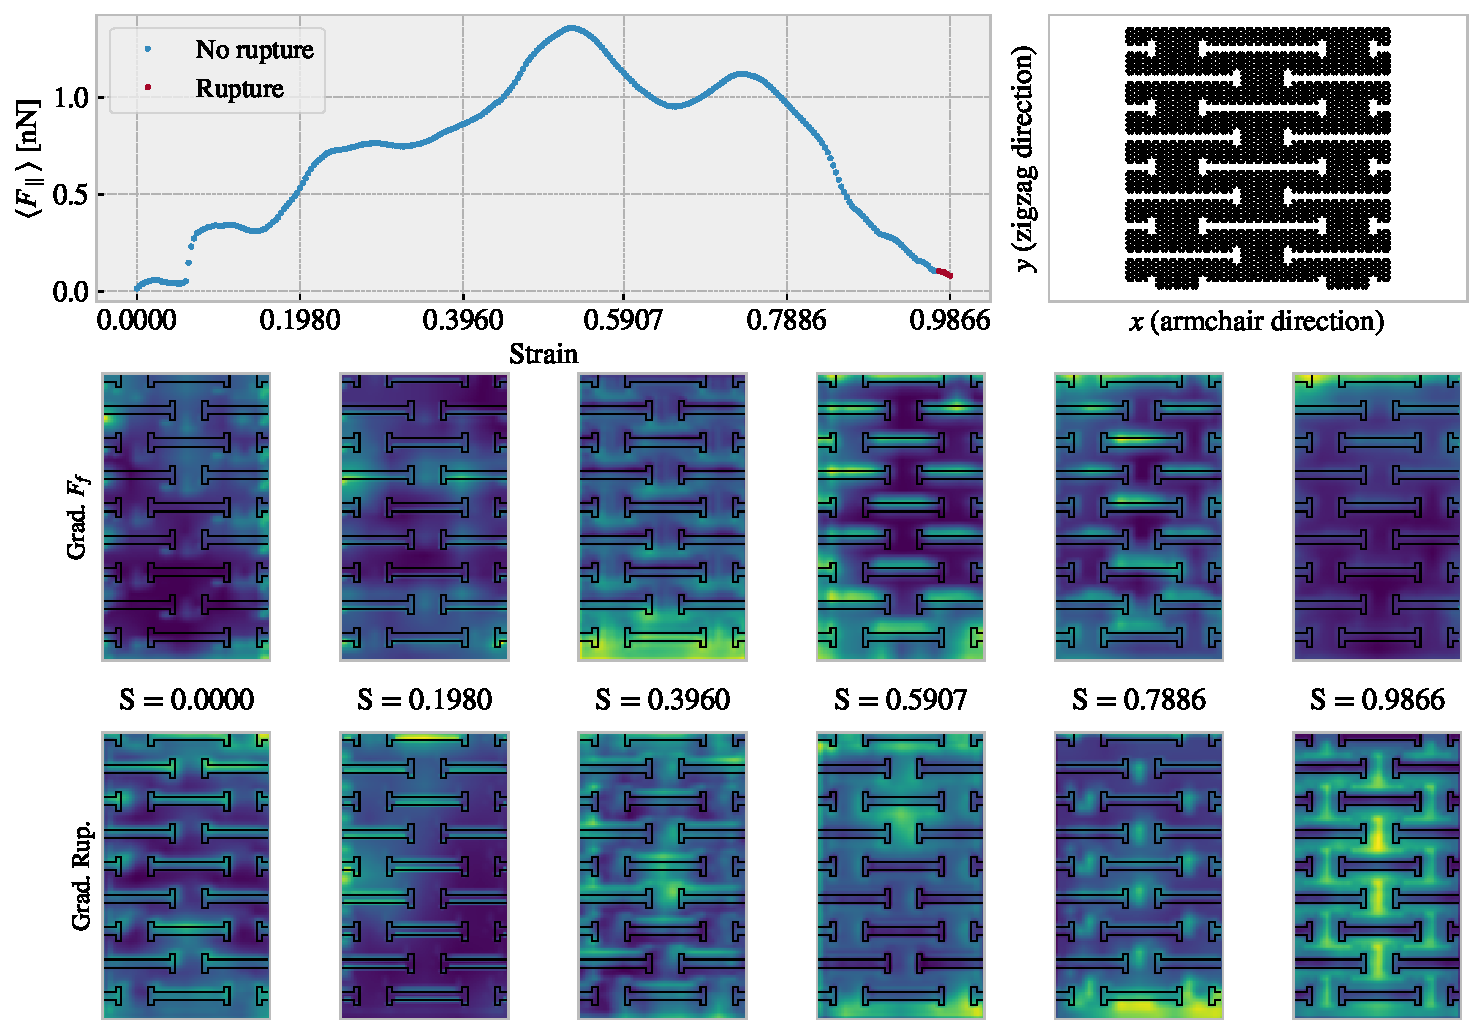
\includegraphics[width=0.8\linewidth]{figures/search/grad_cam_hon_3_3_5_3_12_0.pdf}
  \caption{Honeycomb $(3,3,5,3)$, ref = $(12,0)$}
  \label{fig:GC_hon_search}
\end{figure}  

\begin{figure}[H]
  \centering
  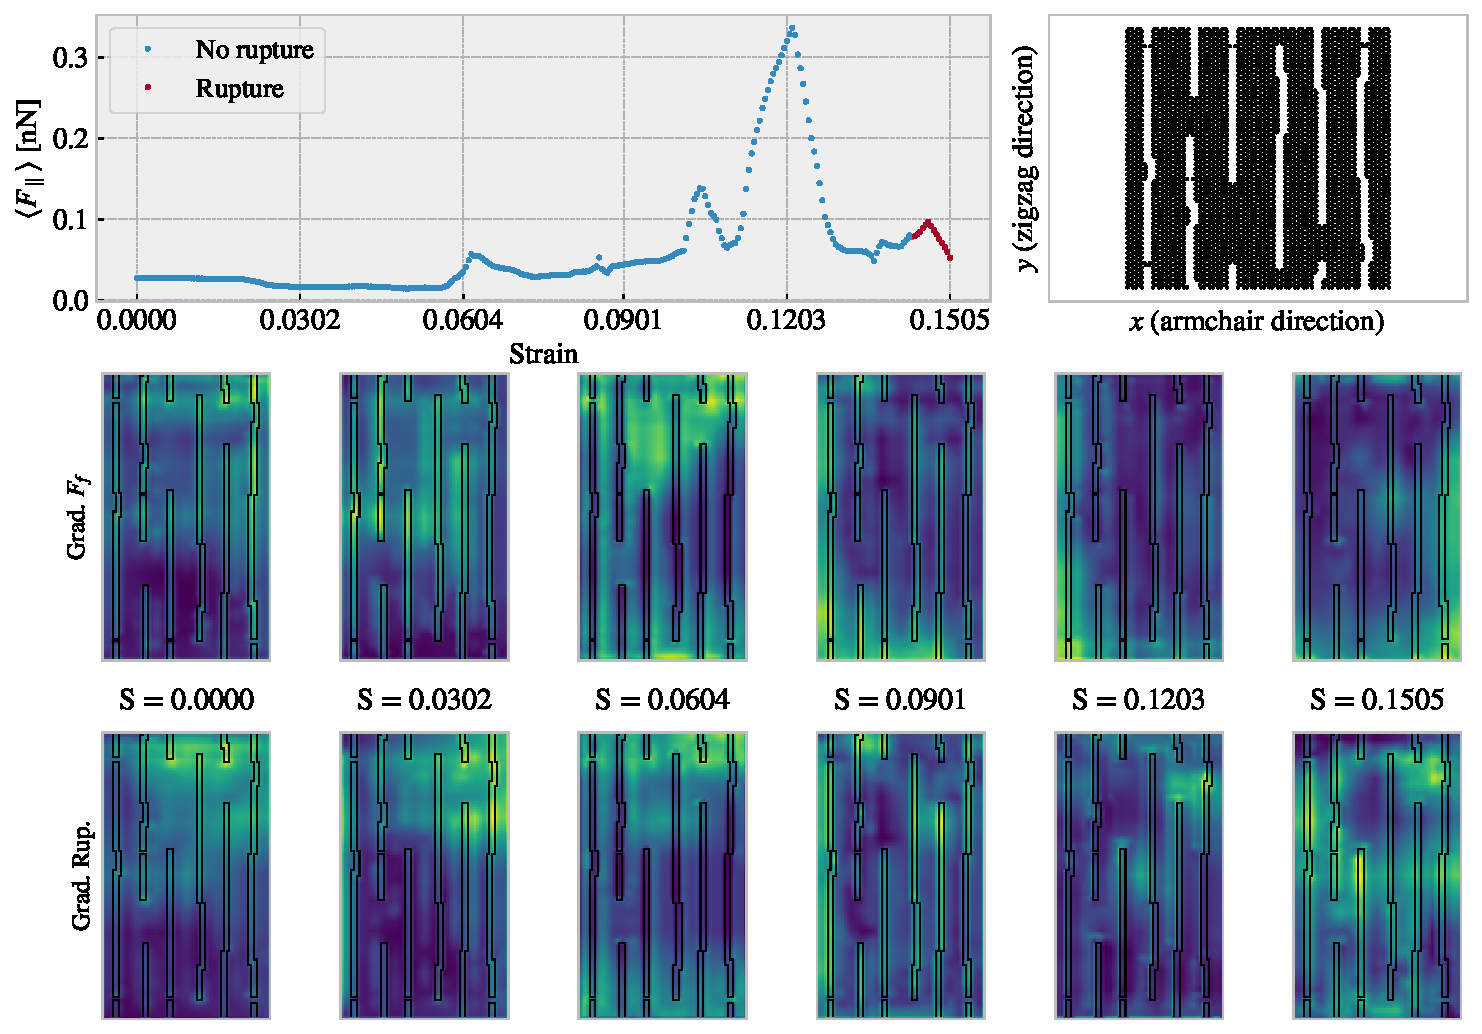
\includegraphics[width=0.8\linewidth]{figures/search/grad_cam_RW_search_max_drop0.pdf}
  \caption{RW.}
  \label{fig:GC_RW_search}
\end{figure}  




% The genetic algorithm approach could possible benefit for a consideration of 2D connections adn translation. It will force any positive patterns to be forced in their location and do not realize that making thoose repeatly will increase effect. It effectively sees every pixel like an unique gene and not really a positional property. 



